% !TEX root = ../main.tex

\chapter{Autonomous Driving Systems}
\label{chapter:AutonomousDrivingSystems}

%* fix the phrasing and continue to expand the current idea
%! fix the paragraph to eventually reflect the full text which encompasses the ADS
This chapter serves to present a more detailed and technical description of previous approaches. The focus will be on their shortcomings to provide a more universal yet safe implementation
of Autonomous Navigational Systems.

\section{Modular Stack}
\label{section:ModularStack}
%* fix and check all citations

Since the early 2000s, researchers and industry manufacturers have adopted the modular stack as the conventional architecture for autonomous vehicles \cite{jain_Autonomy_20_2021, wang_VersatileEfficientReinforcement_2022,tampuu_SurveyEndtoEndDriving_2022}.
The Defense Advanced Research Projects Agency (DARPA) Grand Challenges of 2004 and 2005 accelerated mainstream adoption of the modular stack when teams demonstrated that the modular pipeline could autonomously navigate a demanding off-road desert course within a prescribed time limit \cite{tampuu_SurveyEndtoEndDriving_2022,wang_VersatileEfficientReinforcement_2022,thrun_stanley_2006}.
Engineers described the challenge as solving a software problem, defining deterministic rules and interfaces for each step of the cohesive pipeline \cite{thrun_stanley_2006, montemerlo_winning_2006}.

A robot named Stanley became the first unmanned vehicle to traverse the 212\,km course at the 2005 DARPA Grand Challenge \cite{tampuu_SurveyEndtoEndDriving_2022, hoffmann_AutonomousAutomobileTrajectory_2007, thrun_stanley_2006}.
Stanley's software pipeline is described as comprising of approximately 30 modules organized into six functional layers \cite{tampuu_SurveyEndtoEndDriving_2022, thrun_stanley_2006, montemerlo_winning_2006}.
Fusing input data from various cameras, laser range finders, and other positional sensors, the pipeline routed this stream through the perception layer to construct the surrounding environment and the vehicle's orientation within it \cite{thrun_stanley_2006}.
%? There was no global path planning involved (change: the role of Stanley’s path planner is primarily local obstacle avoidance.)
Achieving high-speed driving yet careful local obstacle avoidance through extensive tweaking: refining software components iteratively, and tuning modules in isolation until the full vehicle exhibited the desired behavior \cite{thrun_stanley_2006, montemerlo_winning_2006}.
This module based development strategy offers clear interpretability and allows engineers to optimize individual units against well-defined inputs and outputs.
%? Talk about more recent benefit of modular stack check Jeremy paper
%? Possible include full extra paragraph here: it was through stanley that established the concrete splits between perception, prediction, planning and control.

However, The DARPA Grand Challenges additionally illustrated the limitations of this approach.
In the 2004 challenge, none of the competing vehicles completed more than 5\% of the course through the Mojave Desert \cite{ogretmen_local_2025, thrun_stanley_2006, montemerlo_winning_2006}.
One year later, only five of the 23 entrants crossed the finish line, indicating that reliable completion of the course still required complex and meticulous tuning for the specific race across the entire software pipeline \cite{tampuu_SurveyEndtoEndDriving_2022,wang_VersatileEfficientReinforcement_2022,jain_Autonomy_20_2021,kocic_end-to-end_2019,thrun_stanley_2006}.
This narrow margin of success is indicative of the error propagation within the modular stack, where modeling approximations and estimation uncertainties accumulate downstream and compound to degrade planning and control performance \cite{jain_Autonomy_20_2021,tampuu_SurveyEndtoEndDriving_2022,wang_VersatileEfficientReinforcement_2022,kocic_end-to-end_2019}.
% \cite{gonzalez_ReviewMotionPlanning_2016,hoffmann_AutonomousAutomobileTrajectory_2007,ogretmen_local_2025,werling_OptimalTrajectoryGeneration_2010,rosero_integrating_2024,thrun_stanley_2006,urmson_autonomous_2008}

\section{End-to-End Neural Network Stack}
\label{section:NNStack}
% \cite{hu_review_2026,tampuu_SurveyEndtoEndDriving_2022,wang_VersatileEfficientReinforcement_2022,kocic_end-to-end_2019,lee_autonomous_2020,hu_learning_2021,chib_recent_2023}

In the end-to-end neural network stack, the entire driving pipeline is collapsed into a single learned task that maps raw sensor data directly to low-level actuator commands or short-horizon trajectories \cite{hu_review_2026, tampuu_SurveyEndtoEndDriving_2022, hu_learning_2021, wang_VersatileEfficientReinforcement_2022, chib_recent_2023}.
This learning based approach has surfaced due to recent innovations of Deep Neural Networks (DNNs) and is often motivated as a solution for the tedious refining process that characterizes modular pipelines \cite{tampuu_SurveyEndtoEndDriving_2022, kocic_end-to-end_2019, hu_learning_2021}.
Rather than relying on hand-crafted interfaces between modules, the network is expected to discover its own latent representations of the task and jointly optimize towards a single downstream objective \cite{tampuu_SurveyEndtoEndDriving_2022, hu_learning_2021, chib_recent_2023}.
In literature, end-to-end driving models are predominantly trained under one of two paradigms: Imitation Learning (IL) and Reinforcement Learning (RL), which are discussed in turn below \cite{hu_review_2026, tampuu_SurveyEndtoEndDriving_2022, wang_VersatileEfficientReinforcement_2022, chib_recent_2023}.

\subsection{Imitation Learning}
\label{subsection:ImitationLearning}

Imitation Learning (IL) frames driving as a supervised learning problem in which the model is trained to reproduce the behavior of an expert human demonstrator \cite{tampuu_SurveyEndtoEndDriving_2022, hu_review_2026, chib_recent_2023}.
During data collection, sensor observations and corresponding expert actions are recorded in pairs.
Convolution Neural Networks (CNNs) are commonly paired with IL models, as they are well suited to processing the high-dimensional visual data produced by the vehicle's cameras \cite{kocic_end-to-end_2019, lee_autonomous_2020, hu_learning_2021}.
CNNs extract spatial features from raw images and condense them into a compact representation that captures the driving scene, which is then mapped onto the corresponding driving action \cite{kocic_end-to-end_2019, hu_learning_2021}.
The network is then optimized to minimize the discrepancy between its own predicted actions and those of the expert over the collected dataset \cite{hu_review_2026, tampuu_SurveyEndtoEndDriving_2022}.
At inference time, the learned policy emits an action based on the current surrounding state, ideally generalizing the demonstrated behavior to previously unseen situations \cite{tampuu_SurveyEndtoEndDriving_2022, kocic_end-to-end_2019}.
Despite this conceptual simplicity, purely imitative policies are well known to suffer from several intertwined limitations.
Consider a driving decision made by the model that directed the car to a situation which was not covered by the initial expert dataset causing the model to malfunction, this is referred to as distribution shift \cite{tampuu_SurveyEndtoEndDriving_2022, wang_VersatileEfficientReinforcement_2022}.
Additionally, data bias and causal confusion describe the possibility of the model to latch onto spurious correlations in the expert demonstrations rather than the true causal structure of the driving task \cite{hu_review_2026, tampuu_SurveyEndtoEndDriving_2022, wang_VersatileEfficientReinforcement_2022, chib_recent_2023}.
These issues are exacerbated by the practical difficulty of curating datasets that are simultaneously large, balanced, and broad enough to cover valid driving scenarios \cite{wang_VersatileEfficientReinforcement_2022, chib_recent_2023}.
This obstacle is particularly pronounced in autonomous racing, where it is nearly impossible to collect data on all possible racing scenarios which could occur, this translates into brittle behavior at the very operating points that matter most on track \cite{wang_VersatileEfficientReinforcement_2022, ogretmen_local_2025}.

\subsection{Reinforcement Learning}
\label{subsection:ReinforcementLearning}
Reinforcement Learning (RL), in contrast, formulates end-to-end driving as a sequential decision-making problem \cite{wang_VersatileEfficientReinforcement_2022, chib_recent_2023, hu_review_2026}.
The agent learns a policy by interacting with its environment and receives rewards based on actions which align with the desired behavior \cite{wang_VersatileEfficientReinforcement_2022, chib_recent_2023}.
Through repeated trial-and-error, the agent gradually converges toward a policy that maximizes the expected cumulative reward, without requiring a curated dataset \cite{wang_VersatileEfficientReinforcement_2022, chib_recent_2023}.
Because the agent actively explores its state-action space, RL relatively more robust to the distribution-shift issue than IL \cite{chib_recent_2023, wang_VersatileEfficientReinforcement_2022}.
In principle, it can also discover unconventional maneuvers that lie outside the support of human driving behavior but are nonetheless dynamically feasible \cite{chib_recent_2023, wang_VersatileEfficientReinforcement_2022}.
This property is particularly attractive for autonomous racing, where exploiting the full capacity of the vehicle is essential \cite{ogretmen_local_2025}.
%* fix example criteria
% Recent work has shown that reward-shaped exploration can recover aggressive yet safe racing styles, and that RL agents can even be used to bias sampling-based planners toward feasible regions of the action space \cite{ogretmen_local_2025, moller_LearningSampleReinforcement2025}.
The absence of labeled data further lowers the barrier to setting up new training scenarios, since reward signals can typically be derived directly from simulator state \cite{wang_VersatileEfficientReinforcement_2022}.
However, RL suffers from poor sample efficiency.
%* fix wording here
RL policies typically demand orders of magnitude more environment interactions than IL requires demonstrations, which in turn ties their development to high-fidelity simulators and considerable computational budgets \cite{wang_VersatileEfficientReinforcement_2022, hu_review_2026}.
Furthermore, exposing RL to high-dimensional sensory inputs, such as raw camera or LiDAR streams, causes the number of possible situations the agent should explore to increase exponentially \cite{wang_VersatileEfficientReinforcement_2022,hu_review_2026,tampuu_SurveyEndtoEndDriving_2022}.
Finally, designing reward functions that faithfully capture the multi-objective and safety-critical nature of driving is equally challenging, as poorly shaped rewards can readily induce reward hacking or unsafe exploration \cite{wang_VersatileEfficientReinforcement_2022, chib_recent_2023}.

Albeit common to both paradigms is the recurring concern that the resulting policies remain difficult to interpret and the arbitrary safety requirements which they inherit, as their decision-making is encoded implicitly within the weights of a deep network rather than in human-readable rules \cite{tampuu_SurveyEndtoEndDriving_2022, wang_VersatileEfficientReinforcement_2022, hu_review_2026, jain_Autonomy_20_2021, jahncke_MINDStackModularInterpretable_2025}.
This opaqueness combined with the data and compute demands outlined above, motivates the hybrid differentiable architectures discussed in the following section.

\section{Modular Differentiable Stack}
\label{section:ModDiffStack}

%! ensure that common points are stated here 

% Speak more on the main concept of modular and differentiable stacks 

% Describe work of DiffStack, and how it operates

% Describe DIPP and how it operates

% Conversely, the modular architecture has matured immensely since that time, where improvements to the system are now introducing neural networks for specific tasks.
% The perception task can highly benefit from Convolution Neural Networks (CNNs) utilizing their ability to extract visual information from images and interpret them.
% The prediction task can also be enhanced with the introduction of a Neural Network which outputs the most probable scenario.
% However, these only achieve partial, unit specific, optimizations rather than a full system optimal point.

% Give examples on this specific topic which includes DiffStack, DIPP, etc.

% What have people used previously
%? Focusing on partial combination of the architectures.
%! Fix this sentence
When discussing the hybrid architecture that is the Modular Differentiable Stack, it is important to consider the previous literature which has lead to this new formulation.
The modular architecture has matured over the years with advancements to the pipeline which utilizes NN to handle some of the tasks individually.
As mentioned previously, Convolution Neural Networks (CNNs) enable extraction of information from images and interpreting them, which the perception task benefits from.
Furthermore, the prediction task can be enhanced by feeding the data into a tailored NN to output the most probable scenario that can occur in the next coming time steps.
Both of these tasks currently are handled in a learning based manner.
%? Include partial combination of NN methods with early exit of the stack to increase interpretability
However, this approach only achieves partial, unit specific optimizations rather than finding a full system optimization.
There have been several varying degrees of hybridization between the modular and end-to-end NN.
The following subsections introduces a handful of the implementations that have had successes in their hybridization.

\subsection{UniAD}
\label{subsection:UniAD}
%* talk about the architecture significance what it considers at important in the paper
%* describe the algorithm and how does it pertain to the differentiability concept
%* what benefits have we achieved from this differentiability, did we perform better?
%* finalize on how this only fulfills partial differentiability as opposed to a fully end-to-end differentiable stack but this is moving in the right direction

% UniAD
% \cite{hu_planning-UniAD_2023}

%? a query is the input vector or token that represents the specific information being sought or the context from which attention is being paid
Hu et al. \cite{hu_planning-UniAD_2023} formulated Unified Autonomous Driving (UniAD), a planning-oriented framework that utilizes multiple transformer based architecture to maneuver through traffic scenarios.
UniAD pursues the familiar perception, prediction, planning task split, but fuses all tasks into one jointly trained neural network whose intermediate modules communicate through shared query interfaces.
%? This framework offers higher interpretability than a standard plain NN by introducing intermediate representation of the encoded data. 
The central design emphases that upstream tasks should not optimize their own local metrics in isolation; instead, every module should be arranged so that its outputs actively support the final ego planning decision.

UniAD ingests a short sequence of multi-camera images and combines them to construct a Bird's-Eye View (BEV) feature map \cite{hu_planning-UniAD_2023}.
From this common representation, four transformer-decoder modules run in sequence, the first two consisting the perception action and the latter two performing prediction.
TrackFormer utilizes BEV to detect and track surrounding agents with learnable track queries.
MapFormer segments map elements in real time such as lanes and road dividers with map queries.
%?  and introduces a dedicated ego-vehicle query that models how the ego vehicle interacts with the rest of the scene.
MotionFormer captures the output of the TrackFormer and MapFormer to forecast future trajectories for each agent in the scene.
OccFormer then predicts future occupancy grids on a per agent basis, giving the planner an explicit notion of where space will become occupied over the next few timesteps.
%! fix phrasing
Finally, a planning head combines the ego query from MotionFormer with a high-level navigation command embedding, attends to the BEV features, and decodes a short-horizon ego waypoint sequence.
%? At inference time, the authors optionally refine this decoded trajectory with a Newton-based collision-avoidance step that pushes the plan away from occupied cells predicted by OccFormer; this refinement operates only during inference and does not participate in the training-time gradient path \cite{hu_planning-UniAD_2023}.

The differentiability mechanism in UniAD is therefore gradient-based co-training through standard backpropagation across the unified network, rather than implicit differentiation through an analytical motion planner.
When the planning loss is applied to the decoded ego waypoints, gradients flow backward through the planning head, MotionFormer, and the preceding perception modules, encouraging TrackFormer, MapFormer, and MotionFormer to produce features that are useful for planning rather than merely strong on their standalone benchmarks \cite{hu_planning-UniAD_2023}.
This is a meaningful form of task coordination, but it differs from the optimization-based differentiability discussed for DiffStack and DIPP: UniAD does not expose a differentiable cost function, learn planner weights, or backpropagate through a sampling or optimal-control solver during training.

Empirically, the planning-oriented organization pays off on the nuScenes benchmark.
In extensive ablations, adding motion forecasting and occupancy prediction before the planner steadily improves planning quality, and the full UniAD stack reduces average planning L2 error from 2.11\,m to 1.03\,m and average collision rate from 0.71\% to 0.31\% compared to the prior vision-based end-to-end method ST-P3 \cite{hu_planning-UniAD_2023}.
UniAD also reports competitive or superior results on tracking, online mapping, motion forecasting, and occupancy prediction relative to prior task-specific baselines such as ViP3D, BEVFormer, and FIERY, even though the authors explicitly note that perception metrics are not the primary target of the design \cite{hu_planning-UniAD_2023}.

UniAD therefore represents a high degree of task hybridization at the architectural level, but only a partial form of the differentiable modular stack pursued in this thesis.
% , leaves the final planning decoder as a learned attention module rather than a differentiable planner with interpretable cost terms, and relies on post-hoc collision refinement at inference.
The framework spans perception and planning inside one network, yet it still omits an explicit low-level controller.
In that sense, UniAD demonstrates that planning-oriented joint training across modular neural heads is valuable, but it does not yet deliver the sensor-to-actuator, optimization-aware differentiability that later systems such as MIND \cite{jahncke_MINDStackModularInterpretable_2025} and DiffPlan \cite{swadiryus_DifferentiableMotionPlanning_2025, koch_DifferentiableInterpretablePath_2025} target on the RoboRacer platform.

\subsection{DiffStack}
\label{subsection:DiffStack}

%* talk about the architecture significance what it considers at important in the paper
%* describe the algorithm and how does it pertain to the differentiability concept
%* what benefits have we achieved from this differentiability, did we perform better?
%* finalize on how this only fulfills partial differentiability as opposed to a fully end-to-end differentiable stack but this is moving in the right direction
% There are varying degrees of hybridization. DiffStack explanation which takes in 
% 1. Prediction is trained for ego planning/control, not generic forecasting. DiffStack reports up to ~15\% higher prediction effectiveness for planning and fewer errors that actually hurt the plan.
% 2. Substantial gains in open-loop and closed-loop planning metrics compared with separately trained modules.
% Joint training beats local training — End-to-end training outperforms training prediction in isolation, even when using handcrafted “planning-aware” auxiliary losses.
% Keeps modularity — Still uses explicit prediction, planning, and control blocks; you get co-optimization without a black-box end-to-end network.
Karkus et al. \cite{karkus_DiffStackDifferentiableModular_2022} propose DiffStack, in which the prediction, planning, and control segment of an urban driving stack is composed of three identifiable modules whose interfaces are kept readable to the engineer, yet whose internal operations are arranged to admit gradients across module boundaries.

The prediction module is a graph-structured Conditional Variational Autoencoder (CVAE).
For each agent in the scene, the encoder ingests the last seconds of state history together with the local map, processes the per-agent histories through Gated Recurrent Unit (GRU) encoders, and aggregates neighbor information via attention over the agent's local interaction graph.
The CVAE then samples from a discrete latent variable and decodes a set of future trajectory hypotheses for each surrounding agent, together with their associated probabilities.
Both the sampling and the decoding are kept differentiable so that gradients arriving from downstream modules can flow back into the GRU encoders.

The planner is a sampling-based trajectory planner that, given the predictions and a goal point, generates $N$ dynamically-feasible candidate trajectories for the ego vehicle \cite{karkus_DiffStackDifferentiableModular_2022}.
Each candidate is scored with a parametric cost $C(\cdot \,; w)$ whose weight vector $w$ is learnable, and the otherwise discrete choice of ``best trajectory'' is relaxed into a soft categorical distribution by passing the negative costs through a softmax.
This softmax-over-costs construction is what makes the discrete trajectory selection differentiable with respect to both the predicted agent states and the cost weights.

The control module is a Model Predictive Controller (MPC) implemented as a box-constrained iterative Linear Quadratic Regulator (iLQR) over a time horizon, using a dynamically extended unicycle model for the ego vehicle \cite{karkus_DiffStackDifferentiableModular_2022}.
Starting from the trajectory selected by the planner, iLQR iteratively forms a quadratic Taylor expansion of the cost and a linear expansion of the dynamics, solves the resulting LQR sub-problem, and updates the control sequence until convergence.
Differentiability of the controller is obtained by implicitly differentiating the Karush--Kuhn--Tucker (KKT) conditions of the final LQR sub-problem, following the differentiable-MPC formulation of Amos et al. \cite{karkus_DiffStackDifferentiableModular_2022}.
The end result is an analytical gradient of the controlled trajectory with respect to the cost weights $w$ and, through the chain rule, with respect to the upstream prediction outputs.

DiffStack is trained on the nuScenes dataset with a composite objective $\mathcal{L} = \mathcal{L}_{\text{pred}} + \mathcal{L}_{\text{plan}} + \mathcal{L}_{\text{ctr}}$, where $\mathcal{L}_{\text{pred}}$ is the original prediction forecasting loss, $\mathcal{L}_{\text{plan}}$ is a cross-entropy that pushes the soft trajectory selection toward the candidate closest to the ground truth, and $\mathcal{L}_{\text{ctr}}$ measures how close the iLQR-controlled trajectory comes to the human reference \cite{karkus_DiffStackDifferentiableModular_2022}.
Because every operator between the controlled trajectory and the prediction parameters is differentiable, $\nabla_\theta \mathcal{L}_{\text{ctr}}$ flows all the way back to the prediction GRU encoders, effectively re-training the prediction module to make the kind of forecasting mistakes that the downstream planner and controller can tolerate.

Empirically, joint training in this fashion yields substantial improvements in both open-loop and closed-loop planning metrics on nuScenes over a baseline that trains the same prediction network in isolation, and even hand-engineered ``planning-aware'' auxiliary losses applied to a non-differentiable stack fall short of the same performance \cite{karkus_DiffStackDifferentiableModular_2022}.
% This gap is informative: it suggests that the cross-module gradient signal carries information about which prediction errors actually matter for driving, and that this information is genuinely difficult to specify by hand.

Unfortunate design choices nevertheless keep DiffStack short of full sensor-to-actuator differentiability.
First, the pipeline begins at the prediction stage rather than at raw sensor data: detection, tracking, and HD-map construction are assumed to already provide clean agent states and a vectorized map, and these upstream perception components stay outside the gradient path.
Second, while the cost weights $w$ are learned, the analytical structure of the cost function and the kinematic model used by iLQR are fixed by the engineer.
DiffStack therefore realizes differentiability across only a slice of the stack, and it leaves the structure of the planner's cost function outside of learning.
% This thesis pushes the gradient chain further in the same direction, in line with MIND \cite{jahncke_MINDStackModularInterpretable_2025} and DiffPlan \cite{swadiryus_DifferentiableMotionPlanning_2025, koch_DifferentiableInterpretablePath_2025}, by extending differentiability toward the sensor side on one end and into additional cost-function parameters of the motion planner on the other.

\subsection{DIPP}
\label{subsection:DIPP}

%* talk about the architecture significance what it considers at important in the paper
%* describe the algorithm briefly and how does it pertain to the differentiability concept
%* what benefits have we achieved from this differentiability, did we perform better?
%* finalize on how this only fulfills partial differentiability as opposed to a fully end-to-end differentiable stack but this is moving in the right direction
% Fixes the prediction-planning split — Explicitly targets the two classic modular failures: isolated prediction/planning and hand-tuned planner costs.
% Joint training beats sequential training — In both open-loop and closed-loop tests, integrated training outperforms using a separately trained prediction module — on both planning and prediction metrics.
% Planning-centric prediction — Predictions are shaped so the planner produces trajectories closer to human driving, not just lower raw forecast error.
% Learned cost function — Planner weights are learned from data instead of manually tuned, improving stability and performance (ablations show learnable components matter).
Huang et al. \cite{huang_DifferentiableIntegratedMotion_2024} propose the Differentiable Integrated Motion Prediction and Planning (DIPP) framework, which also targets the prediction--planning interface but couples the two modules more tightly than DiffStack.
Prediction and planning are fused into a single differentiable computation graph in which the planner's cost function itself is a learnable component.

The input to DIPP is a vectorized representation of the driving scene, consisting of the past state histories of the ego and surrounding agents over a fixed horizon, together with a lane-graph description of the local High-Definition (HD) map \cite{huang_DifferentiableIntegratedMotion_2024}.
A Transformer-based encoder embeds each agent history and each map polyline into a common feature space, and then applies multi-head self-attention and cross-attention to model agent--agent and agent--map interactions.
In contrast to DiffStack, DIPP relies neither on a CVAE nor on a recurrent network for the encoding step; the entire scene context is captured by stacked attention layers operating directly on the vectorized representation.

On top of this shared embedding, a multi-modal decoder produces, for every surrounding agent, a small set of candidate future trajectories together with associated mode probabilities \cite{huang_DifferentiableIntegratedMotion_2024}.
Because the decoder is a feed-forward attention-based network, the predicted trajectories are smooth functions of both the input observations and the scene-encoder parameters, which is what allows them to participate in a differentiable computation graph with the downstream planner.

The planner is formulated as an open-loop, finite-horizon optimal control problem.
A control sequence $u_{1:T}$ is chosen to minimize a composite cost
\begin{equation}
    C\!\left(s_{1:T}, u_{1:T}; \omega\right) = \sum_i \omega_i\, c_i\!\left(s_{1:T}, u_{1:T}, \hat{s}^{\text{pred}}_{1:T}\right),
\end{equation}
where each $c_i$ is a squared residual encoding one driving objective --- for example, progress along the lane, comfort, safety relative to the predicted agent trajectories $\hat{s}^{\text{pred}}_{1:T}$, or adherence to traffic rules --- and each $\omega_i$ is a learnable cost weight \cite{huang_DifferentiableIntegratedMotion_2024}.
The resulting nonlinear least-squares problem is solved with a Gauss--Newton optimizer that iterates over the linearized residuals until convergence.
Because the cost is a sum of differentiable squared residuals and the solver is itself differentiable, gradients of the planned trajectory with respect to both the predicted agent states $\hat{s}^{\text{pred}}_{1:T}$ and the weights $\omega_i$ can be obtained by implicitly differentiating through the Gauss--Newton fixed point \cite{huang_DifferentiableIntegratedMotion_2024}.

DIPP is trained end-to-end on a large urban driving dataset by minimizing an imitation loss between the planned ego trajectory and the recorded human trajectory, augmented with a standard forecasting loss on the surrounding agents \cite{huang_DifferentiableIntegratedMotion_2024}.
A single backward pass updates three coupled sets of parameters at once: the Transformer encoder/decoder weights of the predictor, the cost-function weights $\omega_i$, and the auxiliary prediction heads.
Because every link in the chain from input observations to planned trajectory is differentiable, the imitation loss simultaneously shapes the prediction network so that its forecasts are useful to the planner, and tunes the planner's cost function so that the optimal plan matches the human reference.

Empirically, this jointly trained system outperforms both purely modular baselines and baselines with a separately trained prediction module on a range of open-loop and closed-loop metrics \cite{huang_DifferentiableIntegratedMotion_2024}.
The prediction network is shown to be more accurate exactly where mistakes matter most for planning --- a property the authors term ``planning-centric prediction'' --- and disabling the learnable cost weights in an ablation degrades both stability and final performance, confirming that the differentiable cost function is doing real work rather than acting as an inert hyperparameter.

DIPP therefore makes the cost function itself a learnable component, which is a meaningful step beyond DiffStack on the differentiability axis.
Its gradient chain, however, still begins at the vectorized scene representation and ends at the planned trajectory: detection, tracking, and the construction of the HD-map polylines are assumed upstream and remain outside the gradient path, and so does any low-level controller that would translate the planned trajectory into actuator commands.
The analytical form of each cost residual $c_i$ is also still hand-engineered; only its relative weighting $\omega_i$ is learned.
DIPP thus again achieves only partial sensor-to-actuator differentiability, and the natural extension that this thesis builds upon, in line with MIND \cite{jahncke_MINDStackModularInterpretable_2025} and DiffPlan \cite{swadiryus_DifferentiableMotionPlanning_2025, koch_DifferentiableInterpretablePath_2025}, is to push the gradient chain further --- both toward the sensors and into additional planner-internal parameters --- while preserving the modular, interpretable structure that DIPP and DiffStack are credited with.

\subsection{MIND}
\label{subsection:MIND}
%* talk about the architecture significance what it considers at important in the paper
%* describe the algorithm and how does it pertain to the differentiability concept
%* what benefits have we achieved from this differentiability, did we perform better?
%* finalize on how this only fulfills partial differentiability as opposed to a fully end-to-end differentiable stack but this is moving in the right direction
% MIND Stack
% \cite{jahncke_MINDStackModularInterpretable_2025}
Jahncke and Betz \cite{jahncke_MINDStackModularInterpretable_2025} introduce the Modular, Interpretable, and Differentiable (MIND) software stack, which shifts the hybrid discussion from large-scale urban driving to the RoboRacer / F1TENTH autonomous racing platform used in this thesis.
MIND addresses a gap left by systems such as UniAD, DiffStack, and DIPP: although those frameworks show that joint optimization across modules is beneficial, they either remain perception-heavy urban stacks, stop before actuator commands, or assume clean upstream state estimates rather than learning directly from onboard sensor data under tight embedded compute limits.
MIND instead builds a compact stack around two explicit modules, a learned localization network and a classical Stanley controller, and arranges them so that a downstream control loss can train the upstream localization module beyond pure state estimation.

The MIND pipeline begins with the sensor observations available on the RoboRacer vehicle and passes them through a localization network that estimates the ego pose relative to the track.
Between this network and the controller, the stack exposes human-interpretable intermediate quantities such as lateral cross-track error and heading error relative to the reference path, rather than hiding all reasoning inside a single latent vector \cite{jahncke_MINDStackModularInterpretable_2025}.
These quantities feed directly into a Stanley controller, a well-known geometric path-tracking law that maps cross-track and heading error into steering commands while a separate speed controller regulates longitudinal velocity.
Because the controller is implemented as a fixed analytical law, its operation remains transparent to the engineer even though its outputs participate in end-to-end training.

The differentiability of MIND comes from treating the Stanley controller as a differentiable downstream operator during training.
The stack defines a control loss that measures tracking error along the reference trajectory, and backpropagates this loss through the controller into the localization network \cite{jahncke_MINDStackModularInterpretable_2025}.
As a result, the localization module does not merely minimize pose-estimation error in isolation; it learns representations that reduce the steering and tracking mistakes the controller will actually produce on track.
This is a different hybridization pattern from UniAD's neural task fusion and from DiffStack's gradient path through prediction and MPC: MIND couples raw sensor input to actuator-relevant control error across a very small number of explicit modules, and it does so on real embedded hardware rather than only in offline urban benchmarks.

In their experiments, Jahncke and Betz report that this end-to-end training reduces downstream control loss and yields better tracking performance than state-of-the-art localization baselines trained without the control objective \cite{jahncke_MINDStackModularInterpretable_2025}.
The authors also demonstrate sim-to-real transfer by deploying the jointly trained stack on the physical RoboRacer platform and training localization and controller together toward a single tracking goal under onboard compute constraints \cite{jahncke_MINDStackModularInterpretable_2025}.
For the racing context of this thesis, that result is especially relevant because it shows that differentiable modularity can survive contact with real-time embedded deployment, not just large-scale offline datasets.

MIND nevertheless remains only a partial realization of a full modular differentiable driving stack.
The current version spans localization and control, but it does not yet include prediction, obstacle interaction, or a differentiable motion planner between perception and actuation.
The reference path is assumed to be available, and the stack does not address the richer local replanning problem that becomes necessary when trajectories must be sampled, scored, and selected online during racing.
This limitation directly motivates the subsequent DiffPlan work \cite{swadiryus_DifferentiableMotionPlanning_2025, koch_DifferentiableInterpretablePath_2025}, which extends the MIND philosophy by inserting a differentiable sampling-based motion planner whose cost-function parameters can receive gradients from downstream losses, while still preserving the interpretable modular structure that MIND established on the RoboRacer platform.
Even in its present form, however, MIND is an important step: it proves that partial differentiability can be both interpretable and deployable, and it provides the software foundation on which the motion-planning extensions examined in the remainder of this thesis are built.

\chapter{Motion Planners}
\label{chapter:MotionPlanners}

% Talk about different motion planning techniques. Evolution of motion planning in general to how we reached this current planning task.
% Covering the mathematical background to understand how the sampling planner works.
% Discussion on local planner? differentiable local planner?
% Current reach of stack? what can be achieved now with all the other work having been done?
%* Talk about what a motion planner is, what it does specifically. Why the focus on differentiability.
% \cite{zghair_one_2021,hu_review_2026,orthey_SamplingBasedMotionPlanning_2023,gonzalez_ReviewMotionPlanning_2016,ogretmen_local_2025,koch_DifferentiableInterpretablePath_2025,loganathan_systematic_2023,zhang_IntegratingAlgorithmicSamplingBased_2022}
% \cite{muzzini_GPUImplementationFrenet_2024,olausson_OptimalControlRace_2021,keith_review_2024,werling_OptimalTrajectoryGeneration_2010,naveed_TrajectoryPlanningAutonomous_2021,huang_DifferentiableIntegratedMotion_2024,wursching_SamplingBasedOptimalTrajectory_2021,rosero_integrating_2024,langmann_OnlineVelocityProfile_2025}
%? moving from A to B.
%? what is my goal: traffic? moving boxes? racing?
Motion planning remains one of the most important aspects in unmanned vehicle navigation, encompassing the methods of traversing an environment whether known or unknown.
Navigation can be implemented as a global route to be generally followed by the vehicle or in a local manner where the vehicle constantly updates its own trajectory based on the environment.
The goal of navigation also plays a role in the possible approach of tackling the problem, this could be an autonomous vehicle in an urban environment with traffic with the goal to reach its final destination,
an autonomous mobile robot who's purpose is to transport boxes from one end of a factory to the other, another example would be an autonomous racing vehicle competing against opponents on a closed track with barriers.
Different approaches have been formulated based on the general goal which the autonomous robot needs to achieve. 
This section will provide a review of possible methodologies of solving the path planning problem, covering mainly the rule based and learning based motion planners.

\section{Global and Local Planning}
\label{section:GlobalvsLocal}

%! global planning often comes with a specific objective to achieve, minimum turning, minimum time, what properties does the path need to have.
When it comes to global planning, there comes a predefined and often times precalculated global trajectory which the vehicle follows,
it is the simplest motion planning as it assumes that the surroundings of the vehicle are static, hence the overall predefined map does not change.
Simplifying computations by simply being calculated once and then passed to the vehicle.
The global path can often include details including position, velocity, acceleration, and heading information which the vehicle tries to follow.
Global planning is often formulated as a good initial reference path that the vehicle can consider is "good enough" to use.
This is a perfect use case for factory autonomous mobile robot, if the environment does not change.
When applying to racing scenarios, this is often described as a racing line, a path of a known racing track which under ideal conditions leads to the objective to minimize the lap time of the vehicle.
This can be done because the track is known beforehand and assumes these ideal conditions such as ideal traction, no opponents, no obstacles.

Local motion planning is the iterative process of the vehicle reacting in real time to what the current constrains assigned to it.
Includes obstacle detection, changing conditions of the environment, other AVs in the environment, this involves the dynamic and often stochastic nature of an environment.
The goal of the local motion planner is to redirect and evolve the formulated plan to eventually reach the end point.
It is common to use the global path plan as an initial subsidiary plan, while use online local motion planning to constantly feed updates to the autonomous vehicle.
In racing, this can be interpreted as the driver understanding the dynamic situation they are in and choosing how to react.

\section{Frenet Frame}
\label{section:FrenetFrame}

This section will cover a frame of reference that is commonly used in local motion planning algorithms and is used often in this thesis.

\begin{figure}[htbp]
    \centering
    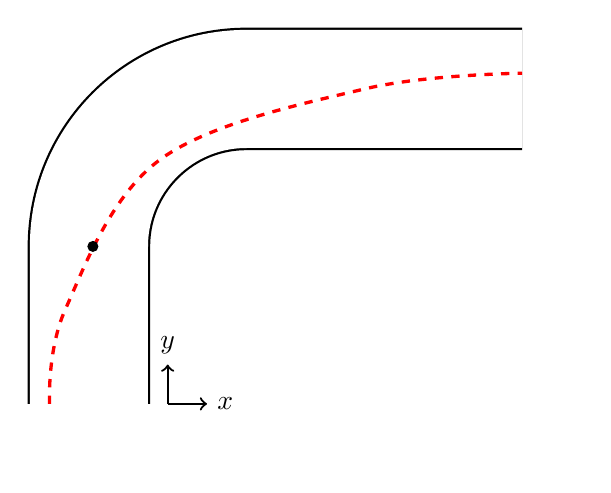
\begin{tikzpicture}
        % Track
        \draw[thick, double=white, double distance=1.5cm] 
            (0, 0) -- (0, 2) arc (180:90:2) -- (5.5, 4);
        % racing line
        \draw[very thick, dashed, red] 
            plot [smooth, tension=0.6] coordinates {(-0.5, 0) (-0.3, 1.2) (0.9, 3.1) (3.5, 4) (5.5, 4.2)};
        % car
        \fill[black] (0.05,2) circle (2pt);
        \draw[->, thick] (1,0) -- (1.5,0) node[right] {$x$};
        \draw[->, thick] (1,0) -- (1,0.5) node[above] {$y$};
    \end{tikzpicture}
    \caption{Track Representation}
    \label{fig:trackrep}
\end{figure}

The Frenet frame of reference is often used when describing a moving particle along a differentiable curve. The use of Frenet coordinate system
$(s, n)$ allows simpler interpretation of curved paths than using a rigid system such as the Cartesian coordinates $(x, y)$.
The curvilinear Frenet frame consists of the longitudinal path $s$ along the curve and its deviation from said curve $n$ or sometimes called $d$.
% modify the phrasing
An additional reason Frenet is beneficial to use is because it simplifies the process of defining planning path constraints or target goals for the vehicle by separating longitudinal and lateral path directions. 
The curve vehicles follow is called a raceline; it is a mathematically optimal line aiming to achieve a certain goal, most commonly fastest time to complete a full lap
around a circuit, or minimum curvature of the raceline. The raceline may be represented as continuous flat curve:

\begin{equation}
    \mathcal{R} = \{ \textbf{r}_{\text{raceline}}(s) \in \mathbb{R}^2 \ | \ s \in [0, s_{\text{lap}}]\},
\end{equation}
where $s$ is the arc-length distance along the raceline curve, and $s_{\text{lap}}$ the total length of a single lap around the circuit. 
The position vector of the reference curve can be described in simple Cartesian coordinates, for each point $s$ on the curve,
\begin{equation}
    \textbf{r}(s) = \begin{bmatrix}
        x_{\text{raceline}} (s) \\ y_{\text{raceline}} (s)
    \end{bmatrix}.
\end{equation}
Additionally, the tangent vector of the raceline defined as the derivative of the position vector with respect to $s$, and the normal vector is orthogonal to the tangent vector, can both be mathematically described as,
\begin{equation}
    \textbf{t}(s) = \frac{d \textbf{r}(s)}{d s} = \begin{bmatrix} \cos (  \psi_{\text{raceline}}(s)) \\ \sin (\psi_{\text{raceline}}(s)) \end{bmatrix}, \qquad
    \textbf{n}(s) = \begin{bmatrix} - \sin (\psi_{\text{raceline}}(s)) \\ \cos (\psi_{\text{raceline}}(s)) \end{bmatrix}.
\end{equation}
Where $\psi (s)$ is the heading angle, relative to the global Cartesian frame, of the raceline at point $s$.

\section{Different Motion Planners}
\label{section:DifferentMotionPlanners}

Rule-based motion planners remain a core component of modular autonomous driving stacks and can be grouped by how they represent and search the configuration space \cite{gonzalez_ReviewMotionPlanning_2016, hu_review_2026, loganathan_systematic_2023}.
The following subsections review three widely used families---graph and search planners, sampling-based planners, and Frenet trajectory sampling---that appear throughout the literature on both urban driving and autonomous racing.
For each family, the principal algorithms, their operating principles, representative deployments, and main limitations are summarized.
A limitation common to all three is emphasized throughout: because they rely on discrete graph expansion, stochastic exploration, or hard selection among candidate trajectories, they are inherently non-differentiable and therefore cannot, in their classical form, propagate gradients from downstream tasks to upstream modules.
This property is central to the motivation for the differentiable planners discussed later in this chapter.

\subsection{Graph and Search Planners}
\label{subsection:GraphandSearch}

Graph and search planners approximate the configuration space as a discrete graph and compute a minimum-cost path from a start state to a goal state \cite{gonzalez_ReviewMotionPlanning_2016, loganathan_systematic_2023}.
The environment is commonly represented as an occupancy grid or state lattice whose nodes correspond to reachable vehicle configurations and whose edges encode valid transitions between them.
Representative algorithms in this family include Dijkstra's algorithm, A*, D* (and its incremental variant D* Lite), and hybrid A*.

Dijkstra's algorithm solves the single-source shortest-path problem by iteratively relaxing edge costs outward from the start node until the goal is reached.
A* extends Dijkstra's search with a heuristic that estimates the remaining cost to the goal, biasing expansion toward promising regions and typically reducing the number of explored nodes.
D* and D* Lite address dynamic environments by efficiently replanning when previously free cells become occupied.
Hybrid A* further combines discrete graph search with continuous vehicle kinematics, connecting lattice nodes through dynamically feasible arcs so that the resulting path respects non-holonomic constraints \cite{gonzalez_ReviewMotionPlanning_2016}.

These methods have been deployed extensively in autonomous driving.
During the DARPA Urban Challenge, Boss used a layered planning architecture whose motion-planning layer combined behavioral reasoning with graph-based search to navigate urban traffic \cite{urmson_autonomous_2008}.
Hybrid A* and lattice-based search were likewise adopted by several Urban Challenge entrants to generate kinematically feasible trajectories in structured road networks \cite{gonzalez_ReviewMotionPlanning_2016}.

The principal drawbacks of graph and search planners are tied to discretization.
Coarse grids can miss narrow passages or produce paths that are not dynamically feasible, whereas fine grids improve resolution at the cost of memory occupancy and query time, which becomes prohibitive over large operational areas \cite{gonzalez_ReviewMotionPlanning_2016, loganathan_systematic_2023}.
Collision checking along candidate edges and the discrete choice of which node to expand next introduce further hard decisions into the pipeline.
From the perspective of differentiable modular stacks, this is a critical limitation: the planner output is a piecewise-constant function of its inputs, so gradients cannot flow through the discrete search and selection steps that define the final path \cite{koch_DifferentiableInterpretablePath_2025, karkus_DiffStackDifferentiableModular_2022}.

\subsection{Sampling-Based Planners}
\label{subsection:SamplingBased}

Sampling-based planners avoid explicit grid construction by randomly probing the configuration space and connecting collision-free samples into a search structure \cite{orthey_SamplingBasedMotionPlanning_2023, gonzalez_ReviewMotionPlanning_2016}.
The most widely used algorithms in this family are the Rapidly-exploring Random Tree (RRT), its asymptotically optimal extension RRT*, and the Probabilistic Roadmap (PRM) method.

RRT incrementally builds a directed tree $G = (V, E)$ rooted at the initial configuration $x_{\text{init}}$.
In each iteration, a random sample $x_{\text{rand}}$ is drawn from the configuration space, the nearest existing node $x_{\text{nearest}}$ is identified, and a new node $x_{\text{new}}$ is created by steering from $x_{\text{nearest}}$ toward $x_{\text{rand}}$ by a bounded step size $\delta$.
The edge $(x_{\text{nearest}}, x_{\text{new}})$ is added to the tree only if the connecting segment passes a collision check.
The process continues until the tree reaches a goal region or a sampling budget is exhausted \cite{orthey_SamplingBasedMotionPlanning_2023}.
RRT* retains this exploration strategy but additionally rewires the tree so that, given sufficient samples, the cost of the returned path converges toward the optimum.
Despite this improvement, practical implementations still trade off sample count against solution quality and real-time latency \cite{orthey_SamplingBasedMotionPlanning_2023, wursching_SamplingBasedOptimalTrajectory_2021}.

Sampling-based methods are attractive for high-dimensional and cluttered environments because they offer probabilistic completeness without requiring a full discretization of the state space \cite{orthey_SamplingBasedMotionPlanning_2023, zhang_IntegratingAlgorithmicSamplingBased_2022}.
They have been applied to highway trajectory planning \cite{zhang_IntegratingAlgorithmicSamplingBased_2022}, urban scenarios with reachable-set pruning \cite{wursching_SamplingBasedOptimalTrajectory_2021}, and local replanning on autonomous race cars \cite{ogretmen_local_2025}.
Recent work has also used reinforcement learning to bias sampling toward regions of the action space that are more likely to yield feasible trajectories, reducing the number of samples required at runtime \cite{moller_LearningSampleReinforcement2025}.

The main limitations of classical sampling-based planners are threefold.
First, standard RRT provides no optimality guarantee, and even RRT* only converges to the optimum as the number of samples grows, which may exceed real-time budgets in safety-critical driving scenarios \cite{orthey_SamplingBasedMotionPlanning_2023}.
Second, uniform or heuristic sampling can produce large numbers of infeasible candidates in complex traffic, wasting computation before a valid trajectory is found \cite{zhang_IntegratingAlgorithmicSamplingBased_2022, wursching_SamplingBasedOptimalTrajectory_2021}.
Third, like graph planners, sampling-based methods are non-differentiable: random sampling, collision-based rejection of edges, and the eventual selection of a single trajectory are discrete operations that block gradient flow to upstream modules \cite{koch_DifferentiableInterpretablePath_2025, karkus_DiffStackDifferentiableModular_2022}.

\subsection{Frenet Trajectory Sampling}
\label{subsection:FrenetSampling}

Frenet trajectory sampling is a local planning approach that generates and evaluates a finite set of candidate trajectories expressed in the curvilinear $(s, n)$ frame introduced in Section~\ref{section:FrenetFrame} \cite{werling_OptimalTrajectoryGeneration_2010, gonzalez_ReviewMotionPlanning_2016}.
Rather than searching a global graph, the planner fixes a reference curve---typically a lane centerline or precomputed raceline---and samples longitudinal and lateral motion relative to that curve.
Each candidate is commonly parameterized as a polynomial in time that satisfies boundary conditions on position and velocity at the planning horizon, after which a cost function scores comfort, progress, collision risk, and adherence to traffic rules \cite{werling_OptimalTrajectoryGeneration_2010}.
The trajectory with the lowest cost is selected for execution.

Werling et al.\ \cite{werling_OptimalTrajectoryGeneration_2010} established this paradigm for dynamic street scenarios, combining long-term behavioral objectives such as lane keeping and merging with reactive collision avoidance in the Frenet frame.
The approach has since been adopted widely in both urban and racing contexts, including GPU-accelerated implementations for embedded F1TENTH platforms \cite{muzzini_GPUImplementationFrenet_2024}, online velocity-aware local planning for autonomous racing \cite{langmann_OnlineVelocityProfile_2025}, and full-scale race-car deployments \cite{ogretmen_local_2025}.
The sampling strategy used in DiffPlan, described in Section~\ref{section:DiffPlanPlanning}, follows the same polynomial-based Frenet formulation.

The strengths of Frenet trajectory sampling are modularity and interpretability: candidate generation, feasibility checking, and cost evaluation are separate, engineer-readable stages, and the separation of longitudinal and lateral motion simplifies constraint specification along curved roads \cite{werling_OptimalTrajectoryGeneration_2010, gonzalez_ReviewMotionPlanning_2016}.
Its drawbacks are equally well documented.
Performance depends strongly on the quality of the reference path; large deviations from the raceline or lane center can invalidate the sampled candidates \cite{langmann_OnlineVelocityProfile_2025}.
Polynomial parameterizations may not fully capture vehicle dynamics, and the number of candidates grows combinatorially with the sampling resolution, creating a tension between coverage and real-time feasibility \cite{werling_OptimalTrajectoryGeneration_2010, muzzini_GPUImplementationFrenet_2024}.
Most importantly for this thesis, selecting the minimum-cost trajectory is a discrete $\arg\min$ operation over a finite candidate set.
As Koch \cite{koch_DifferentiableInterpretablePath_2025} notes for sampling-based planners in general, this hard selection step prevents end-to-end gradient-based training unless the planner is explicitly relaxed, which motivates the differentiable extensions developed in the following subsection.

\subsection{Differentiable Motion Planners}

\chapter{DiffPlan}
\label{chapter:DiffPlan}

%* What does our specific motion planner do?
%* How many parts is it made out of? 
%* How can we describe it
This section will cover the full workings of DiffPlan.
The full architectural sctructure will be explained, including how the algorithm meshes with the simulator and the real car.
Going through the pipeline step by step to explain the steps of how we achieve our objective.

\section{Architecture}

The architectural layout of DiffPlan can be broken down into five major sections of perception, prediction, planning, control, and loss calculation.
The perception unit is carried over from the MIND stack. % describe stack here in detail.
% The RoboRacer platform utilizes Hokuyo UST-10LX 2D LiDAR 
% sensor which introduces a one-dimensional convolution neural network (1D-CNN) designed for LiDAR-based localization on closed-loop tracks.
% The method aims to predict the current vehicle pose by integrating sequential LiDAR scans with encoded information about the previous pose. 
The prediction unit handles obstacle location and rudimentary opponent path prediction.
The planning module samples a variety of short time horizon trajectories along the track, selecting the most optimal path depending on information about ego vehicle and the environment.
The optimally planned path is passed to the differentiable Model Predictive Control (MPC) controller where it is converted to steering and throttle commands to the car.
To complete the evaluation of the plan, a motion model is used to simulate the resulting pose which arises from the control commands posted to the car.
Finally, the loss function is computed at the end which combines all the previous streams of modules to compute a loss component for each module to train them.

\begin{figure}[hb]
    \centering
    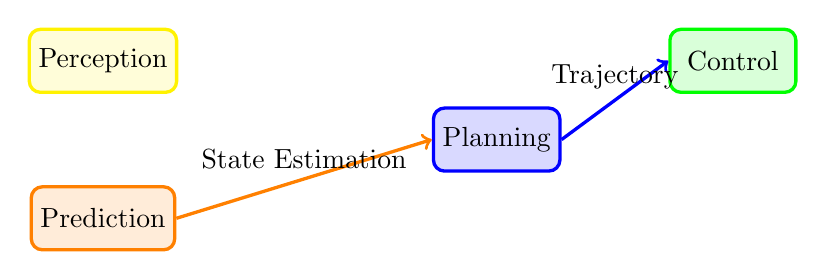
\begin{tikzpicture}
        \node[name=perc, shape=rectangle, draw=yellow, fill=yellow!15, very thick, rounded corners, minimum width=1.6cm, minimum height=0.8cm] at (2, 0) {Perception};
        \node[name=pred, shape=rectangle, draw=orange, fill=orange!15, very thick, rounded corners, minimum width=1.6cm, minimum height=0.8cm] at (2, -2) {Prediction};
        % \draw[->, black, very thick] (sensors.north) -- node[midway, above] {Data} (1.2, -2.3) -- (1.2, 0) -- (perc.north);
        % \node[name=pred, shape=rectangle, draw=orange, fill=orange!15, very thick, rounded corners, minimum width=1.6cm, minimum height=0.8cm, rotate=90] at (5.5, 0) {Prediction};
        % \draw[->, yellow, very thick] (perc.320) -- node[midway, above, black] {Environment} (pred.40);
        % \draw[->, yellow, very thick] (perc.220) -- node[midway, below, black] {Ego Pose} (pred.140);
        \node[name=plan, shape=rectangle, draw=blue, fill=blue!15, very thick, rounded corners, minimum width=1.6cm, minimum height=0.8cm] at (7, -1) {Planning};
        \draw[->, orange, very thick] (pred.east) -- node[midway, above, black] {State Estimation} (plan.west);
        \node[name=ctrl, shape=rectangle, draw=green, fill=green!15, very thick, rounded corners, minimum width=1.6cm, minimum height=0.8cm] at (10, 0) {Control};
        \draw[->, blue, very thick] (plan.east) -- node[midway, above, black] {Trajectory} (ctrl.west);
        % \node[name=act, shape=rectangle, draw=black, fill=gray!15, very thick, rounded corners, minimum width=1.6cm, minimum height=0.8cm, rotate=90] at (10.5,-2.3) {Actuators};
        % \draw[->, black, very thick] (ctrl.south) -- (13.5, 0) -- (13.5, -2.3) -- node[midway, above] {Actuation} (act.south);
    \end{tikzpicture}
    %* fix citation
    \caption{}
    \label{fig:1}
\end{figure}

the DiffPlan stack can interact with two different environments as needed. It can be containerized inside a simulation of the car using a gym to train.
Or it can be placed inside ROS2 to interact with the RoboRacer vehicle and perform in real life. This extends the adaptability of the architecture.

The major objective of DiffPlan is to learn trainable cost weights \(\theta\) that scores trajectory samples. 
The cost weights are then updated using gradient based optimizations.

\section{Perception}
\label{section:DiffPlanPerception}

% Emphasized by the same differentiable naming, DiffLoc is the differentiable localization module used to orient the vehicle in relation to its surroundings.
% Achieved by knitting together LiDAR scan data from the on board sensor with the history of the previous pose of the vehicle.
% This data is ran through a one-dimensional convolution neural network

In the DiffPlan stack, the perception stage is implemented as DiffLoc, the differentiable localization module inherited from the MIND stack \cite{jahncke_MINDStackModularInterpretable_2025, swadiryus_DifferentiableMotionPlanning_2025}.
DiffLoc estimates the vehicle's pose relative to the track from onboard LiDAR measurements.
On the RoboRacer platform, the module consumes scans from a Hokuyo UST-10LX 2D LiDAR sensor together with a short history of previous poses.

The network is built as a one-dimensional convolution neural network followed by fully connected layers that regress the current pose $(\hat{x}, \hat{y}, \hat{\psi})$, consisting of the cartesian position of the vehicle on the track and the global heading of the car respectively \cite{jahncke_MINDStackModularInterpretable_2025, swadiryus_DifferentiableMotionPlanning_2025}.
Localization on closed-loop racetracks is particularly challenging due to the repetitive and recurring geometry as the car laps around the circuit.
The LiDAR can produce highly similar scan patterns at different locations along the circuit.
DiffLoc mitigates this ambiguity by conditioning each prediction with the vehicle's prior pose rather than on the raw scan alone.
The previous pose is first embedded with sinusoidal positional encodings and then discretized onto a spatial grid.
Reducing sensitivity to small pose perturbations and assisting the model to generalize across nearby but non-identical track positions \cite{swadiryus_DifferentiableMotionPlanning_2025}.

During standalone training, DiffLoc is optimized with a mean-squared-error loss between the predicted pose and ground-truth reference values,
\begin{equation}
    \mathcal{L}_{\text{loc}} = \frac{1}{3}\left[(\hat{x} - x)^2 + (\hat{y} - y)^2 + (\hat{\psi} - \psi)^2\right].
\end{equation}
In simulation, the reference pose comes from the training environment; on the physical RoboRacer vehicle, Swadiryus \cite{swadiryus_DifferentiableMotionPlanning_2025} uses a particle-filter estimate as supervision during deployment.
Within the full DiffPlan pipeline, the pose estimate $(x_{\text{est}}, y_{\text{est}}, \psi_{\text{est}})$ serves as the primary input to downstream modules: the planner transforms it into Frenet coordinates before sampling candidate trajectories, and the controller uses the resulting plan to generate steering and throttle commands.
Because DiffLoc remains differentiable during stack training, gradients from downstream planning and control losses can propagate back into the localization network, allowing it to learn pose representations that improve closed-loop driving performance rather than minimizing localization error in isolation \cite{jahncke_MINDStackModularInterpretable_2025, swadiryus_DifferentiableMotionPlanning_2025}.

\section{Prediction}
\label{section:DiffPlanPrediction}

Unlike urban differentiable stacks such as DiffStack or DIPP, DiffPlan does not include a learned multi-agent forecasting module \cite{koch_DifferentiableInterpretablePath_2025, swadiryus_DifferentiableMotionPlanning_2025}.
The original MIND stack likewise omitted prediction entirely, and both Swadiryus and Koch retain only a lightweight environment-modeling stage that supplies the planner with external object information rather than training a dedicated trajectory predictor \cite{jahncke_MINDStackModularInterpretable_2025, swadiryus_DifferentiableMotionPlanning_2025, koch_DifferentiableInterpretablePath_2025}.
In simulation, this stage therefore provides ground-truth positions and planned future waypoints for other traffic participants instead of estimating them from onboard sensors, which isolates planner training from compounding perception and prediction errors \cite{koch_DifferentiableInterpretablePath_2025}.

The prediction interface serves two practical roles in DiffPlan.
For static obstacle avoidance, the planner receives the known locations of obstacles placed around the raceline over a fixed spatial horizon ahead of the ego vehicle.
Because these obstacles remain stationary, their positions can be preprocessed before runtime and reused throughout training and evaluation \cite{swadiryus_DifferentiableMotionPlanning_2025}.
On the physical platform, the same information is obtained from manually placed markers and estimated with a motion-capture system rather than from a learned detector \cite{swadiryus_DifferentiableMotionPlanning_2025}.
For dynamic interaction, DiffPlan implements head-to-head racing against a single opponent agent.
Swadiryus \cite{swadiryus_DifferentiableMotionPlanning_2025} configures this agent as a lead vehicle that follows the same global raceline as the ego car but operates under a reduced velocity cap, creating a standardized overtaking scenario in simulation.
In the FTM Halle head-to-head setup, the opponent is limited to a maximum speed of approximately 1.15~m/s, while the ego vehicle retains its nominal speed range of 2.0~m/s to 3.7~m/s, and both cars are initialized with a fixed longitudinal gap so the trailing vehicle must react to the slower lead car \cite{swadiryus_DifferentiableMotionPlanning_2025}.

Koch \cite{koch_DifferentiableInterpretablePath_2025} extends this scenario for planner co-optimization experiments by equipping the opponent with the same planning architecture as the ego vehicle while still constraining its maximum velocity.
The ego vehicle starts several meters behind the opponent to force repeated overtaking opportunities, and Koch introduces a speed-scaling factor that further limits the lead car when a velocity advantage is needed for safe passing.
The planner consumes the opponent's planned trajectory through the adversary collision cost term, which penalizes ego candidates that approach the lead vehicle's predicted path too closely, and through behavior planning logic that reduces the ego target velocity when a slower car is detected directly ahead \cite{koch_DifferentiableInterpretablePath_2025, swadiryus_DifferentiableMotionPlanning_2025}.
Only vehicles ahead of the ego are considered, assigning right-of-way to the lead car and placing the burden of collision avoidance on the trailing vehicle at each timestep \cite{koch_DifferentiableInterpretablePath_2025}.
Koch demonstrates in head-to-head experiments that the planner can learn cost-weight settings that transition from unsafe following behavior to successful overtaking within a single training lap, even though the opponent model itself remains a simple velocity-capped agent rather than a full interactive prediction module \cite{koch_DifferentiableInterpretablePath_2025}.

In summary, prediction in DiffPlan should be understood as a simplified interaction layer: static obstacles and a single capped-speed opponent provide the planner with the minimum environment context needed for collision-aware local planning and overtaking, without the complexity of a learned multi-modal prediction network.
This design keeps the racing stack focused on differentiable planning and control while leaving full agent forecasting as future work \cite{swadiryus_DifferentiableMotionPlanning_2025, koch_DifferentiableInterpretablePath_2025}.

\section{Planning}
\label{section:DiffPlanPlanning}

% Starting with an initial state of the longitudinal and lateral position and velocity of the vehicle,  respectively.
% A set of sample trajectories are generated constrained by the initial longitudinal velocity and lateral position of the vehicle, the samples terminate at
% the end states, $S_{\text{end}, ij} = [\dot{s}_{\text{end}, i}, n_{\text{end}, j}, \dot{n}_{\text{end}, j}]$ with a specific candidate ${ij}$.

The vehicle now utilizes the information from the two previous modules to start its trajectory planning.
%! mention the planner is based on ogretmen
Given the initial state of the vehicle as a combination of longitudinal, lateral position and velocity, $S_0 = [s_0, \dot{s}_0, n_0, \dot{n}_0]$, respectively.
%? change wording
A set of candidate trajectories are generated constrained by the initial longitudinal velocity and lateral position of the vehicle.
The trajectories terminate at a given time horizon $T$, with each candidate trajectory ${ij}$ assigned an end state $S_{\text{end}, ij} = [\dot{s}_{\text{end}, i}, n_{\text{end}, j}, \dot{n}_{\text{end}, j}]$.
The sampling strategy is split into two sections; the longitudinal sample component followed by the lateral sample component.

%! [WARNING CHANGE LATER] % probably flip the entire description start with what we want to end with. s(t) and the big S matrix 
% The longitudinal sampling is initialized by discretizing the time horizon $T$ into equally spaced steps, a discrete time vector is defined.
% Polynomial functions are used to describe the 
\subsection{Trajectory Generation}
The longitudinal trajectory sampling process is formulated as a boundary-constrained polynomial interpolation problem.
Initialized by discretizing the time horizon $T$ into $N_T$ equally spaced points, defining the discrete time vector $t = \left[t_0, t_1, ..., t_{N_T}\right]$.
This discretization defines the temporal domain over which the candidate trajectories are evaluated.
The boundary conditions encompass the initial longitudinal position $s_{0}$, initial longitudinal velocity $\dot{s}_0$, and the final sampled terminal velocity at the end of the time horizon $\dot{s}_{\text{end}, i}$.
%? a set of feasible terminal velocity conditions is sampled within the predefined velocity range. Each sampled terminal velocity represents a boundary condition for constructing an individual longitudinal trajectory.
The choice of possible values for the final velocity $\dot{s}_{\text{end}, i}$ is important as it ensures the trajectory is kinematic feasible given the initial vehicle state and the raceline's reference speed.
An upper bound is computed as follows;
\begin{equation}
    \dot{s}_{\text{max}} = \text{min}(V_{\text{max}}, \text{max}(\dot{s}_0, \dot{s}_{\text{incr}}) \cdot K ),
\end{equation}
where $K$ is a a scaling factor that accounts for samples to be chosen which can deviation from the raceline, while $V_{\text{max}}$ and velocity increment $\dot{s}_{\text{incr}}$
\begin{equation}
    V_{\text{max}} = \text{min}(V_{\text{target}}, V_{\text{safe}}) \qquad \dot{s}_{\text{incr}} = \text{min}(\dot{s}_0 + \Delta \dot{s}, \dot{s}_{rl}(T)),
\end{equation}
$V_{\text{safe}}$ is a hard cap value the vehicle must not reach. 
an $N_s$ number of end velocity points are sampled with velocities $\{ \dot{s}_{end, i} \}_{i=0}^{N_s}$. 
A quadratic polynomial is selected to describe the longitudinal position profile,
\begin{equation}
    s(t) = c_0 + c_1 t + c_2 t^2 ,
\end{equation}
where $c_0, c_1, c_2$ are unknown coefficients to be computed. The corresponding velocity profile is obtained by differentiating the position polynomial:
\begin{equation}
    \dot{s}(t) = c_1 + 2c_2 t.
\end{equation}
The polynomial coefficient are determined by solving the linear system $A_s c_s = b_s$ where,
\begin{equation}
    A_s = \begin{bmatrix}
        1 & 0 & 0 \\
        0 & 1 & 0 \\
        0 & 1 & 2T
    \end{bmatrix}, \quad
    b_s = \begin{bmatrix}
        s_0 \\
        \dot{s}_0\\
        \dot{s}_i
    \end{bmatrix}.
\end{equation}
With the previously defined constraints $s(0) = s_0, \ \dot{s}(0) = \dot{s}_0, \ \dot{s}(T) = \dot{s}_{\text{end},i}$.
Specifically, the polynomial is constrained to preserve the initial longitudinal position and velocity while reaching the sampled terminal velocity at the end of the time horizon.
% These coefficients ensure that the resulting polynomial maintains continuity with the initial position $s_0$ with the initial velocity $\dot{s}_0$ and a smooth transition to the sampled velocity.
The resulting trajectories form a matrix $S_j \in \mathbb{R}^{N_s \times N_T \times 4}$, such that each row points to trajectory profile $S_i(t)$ elapsed over the time interval $[0, T]$.
%? Since the terminal velocity directly determines the polynomial coefficients, the longitudinal endpoint position is not independently sampled. Instead, it is implicitly determined by the polynomial solution:
% As the final velocities are particularly relevant in racing scenarios, we do not sample the end positions longitudinally [5]; instead, we adjust them according to the polynomial formulation in Eq. 3.18.

Moving to lateral sampling, where the lateral positions are only sampled within the drivable track boundaries,
\begin{equation}
    n_{e,j} \in \left[n_r(s_{e, i}) + \frac{d_w}{2} + \Delta_{\text{safety}}, n_l(s_{e, i}) - \frac{d_w}{2} - \Delta_{\text{safety}}\right],
\end{equation}
with the safety distance $\Delta_{\text{safety}}$ and the vehicle width $d_w$. The lateral positional trajectory is described by the cubic polynomial:
\begin{equation}
    n(t) = c_0 + c_1 t + c_2 t^2 + c_3 t^3,
\end{equation}
and similarly, the lateral velocity $\dot{n}(t)$ corresponds to the first derivative of the positional trajectory.
The unknown polynomial coefficients $c_n = [c_0, c_1, c_2, c_3]^T$ are analogously computed by solving the system of linear equations $A_n c_n = b_n$, where matrix $A_n$ defined as
\begin{equation}
    A_n = \begin{bmatrix}
        1 & 0 & 0 & 0\\
        0 & 1 & 0 & 0\\
        1 & T & T^2 & T^3\\
        0 & 1 & 2T & 3T^2
    \end{bmatrix}, \quad
    b_n = \begin{bmatrix}
        n_0 \\
        \dot{s}_0\\
        n_{e, j} \\
        \dot{n}_{e, j}
    \end{bmatrix}.
\end{equation}
The system can be solved by introducing the constraints $n(0) = n_0, \ \dot{n}(0) = \dot{n}_0 , \ n(T) = n_{\text{end}, j}, \dot{n}(T) = \dot{n}_{\text{end}, j}$.
an $N_n$ number of lateral end points $n_{\text{end}, j}$ are sampled, with the interval split into lateral positions near and far from the raceline.
Consequently, the lateral end velocities must also be calculated based on the longitudinal velocity
\begin{equation}
    \dot{n}_{\text{end}, j} = \dot{s}_{\text{end}, i} \sin (\chi),
\end{equation}
where $\chi$ is the heading angle of the vehicle in the local Frenet Frame.
Therefore, as the lateral trajectory samples are intertwined with their longitudinal counterpart, they must be stored correspondingly in the state matrix $S_{i,j} \in \mathbb{R}^{N_s \cdot N_n \times N_T \times 4}$
% The interval is divided into positions near the raceline (with denser sampling and includes the terminal racing position $n_{rl, i} (T)$) and those farther away, with the total number of samples is denoted as $N_n$.
% The end lateral velocity is chosen based on the longitudinal velocity, calculated as
% \begin{equation}
%     \dot{n}_{e,j} = \dot{s}_{e,i} \sin (\chi),
% \end{equation}
% where $\chi$ is the heading in the local frame. 
% The lateral trajectory samples are stored accordingly to the corresponding longitudinal trajectories, resulting in a state trajectory matrix of $S \in \mathbb{R}^{N_s \cdot N_n \times N_T \times 4}$.

\subsection{Trajectory Assessment}
\label{subsection:TrajectoryAssessment}

Following sample generation, each of the $N$ candidate trajectories is evaluated by a composite cost function that scores several factors: degree of curvature of path, progress, raceline adherence, and collision risk \cite{swadiryus_DifferentiableMotionPlanning_2025, koch_DifferentiableInterpretablePath_2025}.
Swadiryus \cite{swadiryus_DifferentiableMotionPlanning_2025} introduces four interpretable baseline terms with trainable weights, and Koch \cite{koch_DifferentiableInterpretablePath_2025} extends this set to eleven trainable cost-weight parameters by adding slow-driving, wall-proximity, and jitter penalties, as well as nonlinear coupling terms between existing objectives.
For every candidate trajectory, each category $j$ yields a scalar contribution $c_{\text{sample}, j}$, and the planner ranks candidates using a weighted sum over these terms.

\subsubsection{Curvature cost}
The curvature cost encourages smooth trajectories that remain within the vehicle's dynamic limits by penalizing deviations from the reference curvature of the raceline \cite{swadiryus_DifferentiableMotionPlanning_2025, koch_DifferentiableInterpretablePath_2025}.
Swadiryus compares the curvature of the candidate in the velocity frame, $\kappa_{\text{vf}}$, against the raceline curvature $\kappa_{\text{rl}}$.
To avoid penalizing low-speed segments where curvature is dynamically irrelevant, the difference is activated only above a velocity threshold $\tau_c$:
\begin{equation}
    \Delta\kappa_t =
    \begin{cases}
        0 & V_t < \tau_c, \\
        \left|\kappa_{\text{vf}, t}\right| - \left|\kappa_{\text{rl}, t}\right| & V_t \geq \tau_c.
    \end{cases}
\end{equation}
The per-timestep contribution is then
\begin{equation}
    c_{\text{curv}, t} = (\Delta\kappa_t)^2 \cdot \Delta t \cdot \sqrt{V_t},
\end{equation}
and the trajectory-level curvature cost is obtained by summing over the planning horizon, $C_{\text{curv}} = \sum_{t=0}^{T-1} c_{\text{curv}, t}$ \cite{swadiryus_DifferentiableMotionPlanning_2025}.

\subsubsection{Slow-driving cost}
Koch adds a slow-driving cost to reward forward progress independently of the raceline reference velocity \cite{koch_DifferentiableInterpretablePath_2025}.
This term is proportional to the inverse of the average speed along the candidate trajectory and therefore penalizes unnecessarily conservative plans, which is particularly useful during overtaking when the reference velocity may be suboptimal.
% TODO: insert explicit mathematical definition if required by examiner
\begin{equation}
    C
\end{equation}

\subsubsection{Velocity cost}
The velocity cost penalizes deviations from a reference speed profile and keeps the planned motion aligned with the target or raceline velocity \cite{swadiryus_DifferentiableMotionPlanning_2025, koch_DifferentiableInterpretablePath_2025}.
At each timestep, the squared error between the planned speed $V(t)$ and the reference speed $V_{\text{ref}}(t)$ is accumulated:
\begin{equation}
    c_{\text{vel}, t} = \left(V(t) - V_{\text{ref}}(t)\right)^2,
\end{equation}
\begin{equation}
    C_{\text{vel}} = \sum_{t=0}^{T-1} c_{\text{vel}, t} \cdot \Delta t.
\end{equation}
The reference profile depends on the driving context.
If the current speed exceeds the target speed, $V_{\text{ref}}(t)$ follows a deceleration ramp toward the target; otherwise, it tracks the raceline velocity $V_{\text{rl}}(t)$ \cite{swadiryus_DifferentiableMotionPlanning_2025}.
Swadiryus additionally scales penalties for driving below the reference speed with a factor $\lambda_{\text{excess}}$ to discourage unnecessarily slow trajectories \cite{swadiryus_DifferentiableMotionPlanning_2025}.

\subsubsection{Raceline cost}
The raceline cost pulls candidate trajectories toward the precomputed global raceline by penalizing lateral deviation over the planning horizon \cite{swadiryus_DifferentiableMotionPlanning_2025, koch_DifferentiableInterpretablePath_2025}.
Let $d_{\text{rl}}(t)$ denote the lateral offset of the candidate from the reference line at timestep $t$.
Then
\begin{equation}
    c_{\text{rl}, t} = d_{\text{rl}}(t)^2 \cdot \Delta t \cdot F_t,
\end{equation}
\begin{equation}
    C_{\text{rl}} = \sum_{t=0}^{T-1} c_{\text{rl}, t},
\end{equation}
where $F_t$ is a time-scaling factor that increases the influence of later points along the horizon \cite{swadiryus_DifferentiableMotionPlanning_2025}.

\subsubsection{Collision cost}
The collision cost penalizes trajectories that come too close to static obstacles or to the predicted path of an opponent vehicle \cite{swadiryus_DifferentiableMotionPlanning_2025, koch_DifferentiableInterpretablePath_2025}.
Swadiryus evaluates ego and obstacle or opponent trajectories on a common discrete time grid $t_{\text{eq}} = [t_0, t_1, \ldots, t_{N-1}]$ after interpolating all paths into Frenet coordinates.
A collision is detected when both the longitudinal separation $d_s$ and the lateral separation $d_n$ fall below safety margins defined by the vehicle dimensions, buffer zones, and an additional lateral tube term $d_{\text{tube}}$:
\begin{equation}
    d_n < \frac{d_w}{2} + \Delta_{\text{safety}} + d_{\text{tube}}, \qquad d_s < \frac{d_l}{2} + \Delta_{\text{safety}}.
\end{equation}
For trajectories that violate this condition, the cost is computed from the earliest collision time $t_c$, the time-to-collision $\text{TTC} = t_c - t_0$, and the relative velocity $\Delta V$ between ego and the obstacle or opponent:
\begin{equation}
    C_{\text{coll}} = \frac{\Delta V}{\text{TTC}^2}.
\end{equation}
Koch describes the adversary variant of this term more qualitatively as assigning higher cost to trajectories that approach the opponent's planned path too closely, with penalty strength increasing as the distance decreases \cite{koch_DifferentiableInterpretablePath_2025}.

\subsubsection{Wall-proximity cost}
Rather than rejecting wall-intersecting samples with a hard feasibility check, Koch replaces the binary wall constraint with a continuous penalty that grows as a candidate approaches the track boundary \cite{koch_DifferentiableInterpretablePath_2025}.
The wall cost is inversely proportional to the distance from the trajectory to the nearest track wall, encouraging the planner to maintain a safety buffer while still allowing learnable trade-offs between aggression and collision risk.
% TODO: insert explicit mathematical definition if required by examiner

\subsubsection{Jitter cost}
To reduce path oscillations between consecutive planning cycles, Koch includes a jitter penalty that measures the deviation of each candidate from the trajectory selected in the previous timestep \cite{koch_DifferentiableInterpretablePath_2025}.
This term stabilizes control by making the planner prefer spatially consistent plans unless a large improvement in the other cost terms justifies switching to a different maneuver, such as passing an obstacle on the opposite side.
% TODO: insert explicit mathematical definition if required by examiner

\subsubsection{Nonlinear coupling costs}
Koch further introduces four nonlinear coupling terms formed from products of the baseline costs, each with its own trainable weight \cite{koch_DifferentiableInterpretablePath_2025}:
velocity--curvature, velocity--wall proximity, curvature--wall proximity, and velocity--curvature--wall proximity.
These terms model coupled failure modes that linear penalties cannot capture on their own, such as high lateral acceleration near a wall or traction loss under combined speed and curvature.
% TODO: insert explicit product formulations if required by examiner

\subsubsection{Total scalar cost}
After computing the category-level costs for a candidate trajectory, the planner assigns a single scalar score by weighting and summing all active terms.
In the notation used by Koch, each category $j$ contributes $c_{\text{sample}, j}$ and is scaled by a trainable parameter $\theta_j$:
\begin{equation}
    C_{\text{sample}} = \sum_j \theta_j \, c_{\text{sample}, j}.
    \label{eq:DiffPlanTotalCost}
\end{equation}
Swadiryus uses the same weighted-sum structure with weights $w_j$ on the four baseline terms $C_{\text{curv}}$, $C_{\text{vel}}$, $C_{\text{rl}}$, and $C_{\text{coll}}$ \cite{swadiryus_DifferentiableMotionPlanning_2025}.
To keep the three trajectory-quality weights balanced during optimization, Swadiryus normalizes the curvature, velocity, and raceline weights with a temperature-scaled softmax so that they form a convex combination:
\begin{equation}
    w_i = \frac{\exp(w_{\text{init}, i} / \tau)}{\sum_{k \in \{\text{curv}, \text{vel}, \text{rl}\}} \exp(w_{\text{init}, k} / \tau)}, \qquad i \in \{\text{curv}, \text{vel}, \text{rl}\},
\end{equation}
while the collision weight remains unconstrained so that safety can be scaled independently \cite{swadiryus_DifferentiableMotionPlanning_2025}.
Koch extends this idea to eleven trainable parameters $\theta_j$ covering the additional linear and nonlinear terms, and the candidate with the lowest $C_{\text{sample}}$ is passed to the differentiable sample-selection stage described in Section~\ref{subsection:SampleSelection} \cite{koch_DifferentiableInterpretablePath_2025}.

\subsection{Sample Selection}
\label{subsection:SampleSelection}

After trajectory assessment, DiffPlan must select one candidate from the sampled set for execution.
In the classical formulation, this step is a discrete $\arg\min$ over the scalar costs $C_{\text{sample}, i}$, which is non-differentiable: a small change in a cost weight $\theta_j$ usually leaves the selected index unchanged, producing zero gradient, or abruptly switches the selection, producing a discontinuous jump \cite{koch_DifferentiableInterpretablePath_2025}.
This breaks the end-to-end gradient path from downstream control and loss terms back into the trainable planner weights, which is why Koch \cite{koch_DifferentiableInterpretablePath_2025} replaces hard selection with a differentiable relaxation.

%! fix this 
Koch evaluates several candidate methods for this purpose \cite{koch_DifferentiableInterpretablePath_2025}.
An identity straight-through estimator (STE) preserves the correct forward pass by selecting the minimum-cost trajectory, but it routes downstream gradients through the selected sample in a way that no longer reflects how the loss depends on the candidate costs, making the update signal largely meaningless.
A weighted average (WA) relaxation instead produces meaningful gradients by softening the selection, but its forward pass returns a mixture of trajectories rather than a single feasible plan; when viable candidates pass an obstacle on opposite sides, their average can lie inside the obstacle and become physically invalid \cite{koch_DifferentiableInterpretablePath_2025}.
% Sample-inefficient alternatives such as stochastic smoothing and REINFORCE-style score-function estimators are also considered, but rejected because DiffPlan is intended to train both in simulation and on the embedded vehicle, where repeated stack rollouts per timestep are too expensive \cite{koch_DifferentiableInterpretablePath_2025}.

Koch therefore adopts Straight-Through-Gumbel-Softmin, which combines the strengths of STE and WA \cite{koch_DifferentiableInterpretablePath_2025}.
In the forward pass it behaves like discrete selection and outputs the lowest-cost candidate, preserving safe and interpretable planner behavior.
In the backward pass it behaves like a softened weighted average over candidates, allowing gradients to flow back into the cost weighting and therefore into the trainable parameters $\theta_j$ \cite{koch_DifferentiableInterpretablePath_2025}.

Let $S \in \mathbb{R}^{N \times D}$ denote the matrix of $N$ candidate trajectories and $\mathbf{c} \in \mathbb{R}^{N}$ the corresponding cost vector after Eq.~\eqref{eq:DiffPlanTotalCost}.
Straight-Through-Gumbel-Softmin proceeds as follows \cite{koch_DifferentiableInterpretablePath_2025}:

\begin{algorithm}[ht!]
\caption{Differentiable Sample Selection}
    \begin{algorithmic}[1]
    \Require candidate trajectories $S$, cost vector $c$, temperature $\tau > 0$
    % \Ensure Position trajectories $\mathbf{S}$, velocity trajectories $\dot{\mathbf{S}}$, end positions $\mathbf{s}_{end}$
    \State $u \gets \text{RANDOM}(0, 1)$ \Comment{take random sample from uniform distribution}
    \State $g \gets - \ln (- \ln (u))$
    \State $\tilde{c} \gets c + \tau g$
    \State $y_{\text{soft}} \gets \text{softmin}(\frac{\tilde{c}}{\tau})$
    \State $k \gets \text{argmin}(\tilde{c})$
    \State Initialize $y_{\text{hard}}$ as a vector of ones with the size of $k$
    \State $y_{\text{select}} \gets sg[y_{\text{hard}} - y_{\text{soft}}] + y_{\text{soft}}$
    \State $s_{\text{select}} \gets S^T y_{\text{select}}$
    \State \Return $s_{\text{select}}$
\end{algorithmic}
\end{algorithm}

% ! fix this
\begin{enumerate}
    \item Draw uniform noise $u \sim \mathcal{U}(0,1)$ and convert it to Gumbel noise $g = -\ln(-\ln u)$.
    \item Form perturbed costs $\tilde{\mathbf{c}} = \mathbf{c} + \tau g$, where $\tau > 0$ is a temperature parameter.
    \item Compute the soft selection vector $\mathbf{y}_{\text{soft}} = \text{softmin}(\tilde{\mathbf{c}} / \tau)$.
    \item Identify the hard winner $k = \arg\min_i \tilde{c}_i$ and set $\mathbf{y}_{\text{hard}} = \mathbf{1}_k$.
    \item Combine both with the straight-through trick
    \begin{equation}
        \mathbf{y}_{\text{select}} = \text{sg}[\mathbf{y}_{\text{hard}} - \mathbf{y}_{\text{soft}}] + \mathbf{y}_{\text{soft}},
    \end{equation}
    where $\text{sg}[\cdot]$ stops gradients through the hard term during backpropagation.
    \item Return the selected trajectory $s_{\text{select}} = S^{\top}\mathbf{y}_{\text{select}}$.
\end{enumerate}
During the forward pass, the stop-gradient term makes $\mathbf{y}_{\text{select}} = \mathbf{y}_{\text{hard}}$, so the planner executes exactly one candidate trajectory.
During the backward pass, gradients flow through $\mathbf{y}_{\text{soft}}$, approximating how downstream loss would change if each candidate contributed more or less to the selection \cite{koch_DifferentiableInterpretablePath_2025}.

The temperature $\tau$ controls exploration and gradient spreading.
A larger $\tau$ increases the influence of Gumbel noise in the forward pass, occasionally selecting suboptimal trajectories and allowing more candidates to receive non-negligible gradients in the backward pass.
A smaller $\tau$ makes selection sharper and concentrates gradient flow on the lowest-cost candidates \cite{koch_DifferentiableInterpretablePath_2025}.
With this mechanism in place, the selected trajectory can be passed to the differentiable controller while preserving a continuous gradient path through the planner's cost weights.

\section{Control}
\label{section:DiffPlanControl}

The control module closes the loop between planning and actuation by converting the selected local trajectory into steering and throttle commands that the vehicle can execute \cite{swadiryus_DifferentiableMotionPlanning_2025, koch_DifferentiableInterpretablePath_2025}.
At each timestep, the controller compares the current vehicle state with the reference defined by the planner and computes control inputs that reduce tracking error.
Longitudinal control regulates speed, acceleration, and braking, while lateral control adjusts steering to follow the planned path \cite{swadiryus_DifferentiableMotionPlanning_2025}.

Controllers in autonomous driving are commonly grouped into three families \cite{ogretmen_local_2025, swadiryus_DifferentiableMotionPlanning_2025}.
Classic controllers rely on fixed analytical laws such as PID or geometric path-tracking methods.
Optimization-based controllers solve a constrained optimal-control problem over a receding horizon, with Model Predictive Control (MPC) as the most prominent example.
Learning-based controllers instead infer control policies from data or environment interaction, optionally hybridized with model-based methods.
DiffPlan adopts an optimization-based controller in the form of Differentiable MPC (DiffMPC), which tracks the planner reference while remaining compatible with end-to-end gradient-based training \cite{swadiryus_DifferentiableMotionPlanning_2025, koch_DifferentiableInterpretablePath_2025, tungka_diffmpc_2024}.

\subsection{Differentiable Model Predictive Control}
\label{subsection:DiffMPC}

Differentiable MPC extends classical MPC so that gradients of the optimized control sequence can flow back to reference trajectories, model parameters, and upstream planner outputs \cite{amos_differentiable_2018, swadiryus_DifferentiableMotionPlanning_2025, koch_DifferentiableInterpretablePath_2025}.
Amos et al.\ \cite{amos_differentiable_2018} formulate this problem for integration into end-to-end learning pipelines, and Tungka implements a DiffMPC module for the RoboRacer stack using the Locus Lab MPC solver together with PyPose \cite{wang_pypose_2023, tungka_diffmpc_2024}.

At each control step, MPC solves a finite-horizon optimization over predicted states and inputs.
Given state $x_t \in \mathbb{R}^n$, control input $u_t \in \mathbb{R}^m$, dynamics $x_{t+1} = f(x_t, u_t)$, and stage cost $C_t(x_t, u_t)$, the receding-horizon problem is
\begin{equation}
    \min_{(x_t, u_t)_{t=1}^{T}} \sum_{t=1}^{T} C_t(x_t, u_t)
    \quad \text{subject to} \quad
    x_{t+1} = f(x_t, u_t), \quad x_1 = x_{\text{init}}, \quad u_t \in \mathcal{U}, \quad x_t \in \mathcal{X},
\end{equation}
where $\mathcal{U}$ and $\mathcal{X}$ denote admissible input and state sets and only the first optimized input is applied before the problem is solved again at the next timestep \cite{swadiryus_DifferentiableMotionPlanning_2025}.
A common quadratic tracking objective penalizes deviation from the planner reference $r_{t+k}$ and excessive control changes:
\begin{equation}
    J = \sum_{k=0}^{N} (y_{t+k} - r_{t+k})^{\top} Q (y_{t+k} - r_{t+k})
    + \sum_{k=0}^{M} \Delta u_{t+k}^{\top} R \Delta u_{t+k},
\end{equation}
where $Q$ and $R$ weight tracking error and control smoothness, and $\Delta u_{t+k} = u_{t+k} - u_{t+k-1}$ \cite{swadiryus_DifferentiableMotionPlanning_2025}.

Classical MPC is effective for trajectory tracking but its solver is not differentiable by default, which prevents end-to-end co-training with perception or planning modules \cite{amos_differentiable_2018, swadiryus_DifferentiableMotionPlanning_2025}.
Differentiable MPC addresses this by differentiating through the optimizer's fixed point.
For the linear-quadratic case, the optimal state-control sequence $\tau_t = [x_t, u_t]$ satisfies
\begin{equation}
    \tau_{1:T}^{*} = \arg\min_{\tau_{1:T}} \sum_{t=1}^{T} \left(\frac{1}{2}\tau_t^{\top} C_t \tau_t + c_t^{\top}\tau_t\right)
    \quad \text{subject to} \quad x_{t+1} = F_t \tau_t + f_t, \quad x_1 = x_{\text{init}},
\end{equation}
and gradients of a downstream loss $\ell(\tau^{*})$ with respect to problem parameters $\theta = \{C, c, F, f\}$ follow the chain rule
\begin{equation}
    \frac{\partial \ell}{\partial \theta} = \frac{\partial \ell}{\partial \tau^{*}} \frac{\partial \tau^{*}}{\partial \theta}.
\end{equation}
The backward pass can be implemented as another LQR problem that reuses the Riccati factorization from the forward solve \cite{amos_differentiable_2018, swadiryus_DifferentiableMotionPlanning_2025}.

For nonlinear vehicle dynamics, non-quadratic costs, and box constraints on inputs, DiffMPC iteratively linearizes the dynamics and quadratizes the cost, then solves the resulting subproblem with iterative LQR (iLQR) until convergence \cite{amos_differentiable_2018, swadiryus_DifferentiableMotionPlanning_2025, tungka_diffmpc_2024}.
Gradients are obtained from the final convexified problem at the solver fixed point, enabling the controller to participate in the same end-to-end training loop as DiffPlan's planner and localization modules \cite{koch_DifferentiableInterpretablePath_2025, swadiryus_DifferentiableMotionPlanning_2025}.
Koch \cite{koch_DifferentiableInterpretablePath_2025} adopts DiffMPC in the modified stack to improve tracking quality and provide stronger gradients during planner co-optimization.

% \subsection{Differentiable Model Predictive Control}
% \cite{amos_differentiable_2018,wang_pypose_2023,tungka_diffmpc_2024}
% The controller responsible for ensuring that the system follows a desired trajectory or maintains a specific state by continuously adjusting control inputs.
% comparing the system's current state with the desired state defined by the planner and define actions to minimize the resulting error.
% ...
\subsection{Motion Model}

%! fix
The differentiable motion model completes the forward evaluation of DiffPlan.
Given the current vehicle pose and the steering and velocity commands output by DiffMPC, pose estimates are propagated over the next two timesteps.
The model uses pose $(x, y, \theta)$ for position and heading, longitudinal velocity $v$, and steering angle $\delta$.
Vehicle geometry is defined by the distances from the center of gravity to the front and rear axles,
$\ell_f$ and $\ell_r $, and the wheelbase $L_{\mathrm{wb}}$.
Heading angles are wrapped to $(-\pi, \pi]$ via $\mathrm{wrap}(\alpha) = ((\alpha + \pi) \bmod 2\pi) - \pi$.
At the first timestep,
\begin{equation}
    \begin{aligned}
        x_1 &= x + v\cos(\theta)\Delta t_1, \\
        y_1 &= y + v\sin(\theta)\Delta t_1, \\
        \theta_1 &= \mathrm{wrap}\!\left(\theta + \frac{v\tan(\delta)}{L_{\mathrm{wb}}}\Delta t_1\right).
    \end{aligned}
\end{equation}
At the second timestep,
\begin{equation}
    \begin{aligned}
        x_2 &= x_1 + v\cos(\theta_1)\,\Delta t_2, \\
        y_2 &= y_1 + v\sin(\theta_1)\,\Delta t_2, \\
        \theta_2 &= \mathrm{wrap}\!\left(\theta_1 + \frac{v\tan(\delta)}{L_{\mathrm{wb}}}\,\Delta t_2\right).
    \end{aligned}
\end{equation}
The resulting estimated pose is used to calculate the cross-track and heading error for the control loss.
This enables end-to-end gradient flow, allowing the localization module to be trained on the control loss.

\section{Loss Formulation}
\label{section:LossFormulation}

The loss function closes the end-to-end training loop of DiffPlan.
At each control timestep, the stack executes a forward pass through localization, planning, control, and---in Koch's extended formulation---a differentiable motion model that propagates the estimated vehicle pose over the next two timesteps \cite{swadiryus_DifferentiableMotionPlanning_2025, koch_DifferentiableInterpretablePath_2025}.
The resulting supervisory signal is a weighted sum of module-specific terms whose gradients flow backward through every differentiable stage, enabling co-optimization of localization parameters, planner cost weights, and---where the gradient path is unbroken---controller behavior \cite{swadiryus_DifferentiableMotionPlanning_2025, koch_DifferentiableInterpretablePath_2025}.

\subsection{Composite Objective}

Swadiryus \cite{swadiryus_DifferentiableMotionPlanning_2025} defines the baseline DiffPlan training objective as a weighted combination of localization, planning, and control losses:
\begin{equation}
    \mathcal{L}_{\text{total}} = \alpha_{\text{loc}}\,\mathcal{L}_{\text{loc}} + \alpha_{\text{plan}}\,\mathcal{L}_{\text{plan}} + \alpha_{\text{ctr}}\,\mathcal{L}_{\text{ctr}},
    \label{eq:DiffPlanTotalLoss}
\end{equation}
where $\alpha_{\text{loc}}$, $\alpha_{\text{plan}}$, and $\alpha_{\text{ctr}}$ are scalar weighting factors that set the relative importance of each module during optimization.
In end-to-end training, Swadiryus uses $\alpha_{\text{loc}} = 1.0$, $\alpha_{\text{plan}} = 0.3$, and $\alpha_{\text{ctr}} = 5.0$ for the cross-track component of the control loss \cite{swadiryus_DifferentiableMotionPlanning_2025}.
When training the planner in isolation with ground-truth pose estimates, only $\alpha_{\text{plan}}$ is nonzero \cite{swadiryus_DifferentiableMotionPlanning_2025}.

Koch \cite{koch_DifferentiableInterpretablePath_2025} retains the same additive structure but replaces the decoupled planner-centric supervision of Swadiryus with control-driven terms that rate the executed vehicle state rather than the planned trajectory alone.
The total loss is therefore expressed as
\begin{equation}
    \mathcal{L}_{\text{total}} = \sum_i \alpha_i\,\mathcal{L}_i,
    \label{eq:KochTotalLoss}
\end{equation}
where each $\mathcal{L}_i$ encodes one driving objective and the coefficients $\alpha_i$ are chosen per experiment.
Because Koch couples the loss to the pose predicted by the motion model after DiffMPC, gradients can propagate through control, differentiable sample selection, and the planner cost weights $\theta_j$ in a single backward pass---the end-to-end training mode that Swadiryus's original stack could not fully exploit due to non-differentiable trajectory selection \cite{swadiryus_DifferentiableMotionPlanning_2025, koch_DifferentiableInterpretablePath_2025}.

\subsection{Localization Loss}

The localization loss supervises DiffLoc during both standalone pretraining and joint stack optimization \cite{swadiryus_DifferentiableMotionPlanning_2025, jahncke_MINDStackModularInterpretable_2025}.
Given predicted pose $(\hat{x}, \hat{y}, \hat{\psi})$ and ground-truth reference $(x, y, \psi)$, the objective is the mean squared error
\begin{equation}
    \mathcal{L}_{\text{loc}} = \frac{1}{3}\left[(\hat{x} - x)^2 + (\hat{y} - y)^2 + (\hat{\psi} - \psi)^2\right].
    \label{eq:DiffPlanLocLoss}
\end{equation}
During stack training, gradients from downstream planning and control losses additionally shape the localization network toward pose estimates that reduce tracking error rather than minimizing Eq.~\eqref{eq:DiffPlanLocLoss} in isolation \cite{jahncke_MINDStackModularInterpretable_2025, swadiryus_DifferentiableMotionPlanning_2025}.

\subsection{Planner Loss}

Swadiryus introduces a planner-specific loss that evaluates the quality of the selected trajectory in isolation from closed-loop execution \cite{swadiryus_DifferentiableMotionPlanning_2025}.
Let $C_j$ denote the scalar contribution of planner cost category $j$ for the lowest-cost candidate after Eq.~\eqref{eq:DiffPlanTotalCost}, and let $w_j$ be the corresponding trainable weight.
The planner loss combines the weighted plan cost with a regularization term that discourages the optimizer from driving unused weights to zero:
\begin{equation}
    \mathcal{L}_{\text{plan}} = \sum_j w_j\, C_j + \sum_j (1 - w_j)^2\, C_j.
    \label{eq:DiffPlanPlanLoss}
\end{equation}
The second term penalizes vanishing weights on cost categories that still carry nonzero cost, preventing the model from artificially reducing $\mathcal{L}_{\text{plan}}$ by collapsing $w_j \to 0$ instead of improving trajectory quality \cite{swadiryus_DifferentiableMotionPlanning_2025}.
In Swadiryus's implementation, $\mathcal{L}_{\text{plan}}$ is the primary signal for updating planner cost weights $w_j$, because gradients from the control loss do not propagate through the planner to the cost parameters \cite{swadiryus_DifferentiableMotionPlanning_2025}.
Koch retains $\mathcal{L}_{\text{plan}}$ only for benchmarking: it scores the $\theta_j$-weighted optimal plan cost without simulating the vehicle response and is not used as the main training signal in the end-to-end experiments \cite{koch_DifferentiableInterpretablePath_2025}.

\subsection{Control Loss}

Swadiryus formulates the control loss from tracking errors computed on the executed vehicle state relative to the planner reference \cite{swadiryus_DifferentiableMotionPlanning_2025}.
Let $e_{\text{ct}}$ denote the cross-track error, $\psi$ the current heading, $\psi_{\text{ref}}$ the reference heading, and $\theta_t$ the orientation at timestep $t$.
Then
\begin{equation}
    \mathcal{L}_{\text{ctr}} = \alpha_{\text{ct}}\, e_{\text{ct}}^{2} + \alpha_{h}\,|\psi - \psi_{\text{ref}}| + \alpha_{o}\,|\theta_t - 2\theta_{t-1} + \theta_{t-2}|,
    \label{eq:DiffPlanCtrlLoss}
\end{equation}
where the first term penalizes lateral deviation from the reference path, the second penalizes heading mismatch, and the third is a second-order finite difference that discourages abrupt orientation changes \cite{swadiryus_DifferentiableMotionPlanning_2025}.
Typical weightings are $\alpha_{\text{ct}} = 5$, $\alpha_{h} = 0$, and $\alpha_{o} = 1$ \cite{swadiryus_DifferentiableMotionPlanning_2025}.

Koch does not use Eq.~\eqref{eq:DiffPlanCtrlLoss} directly as the downstream supervisory signal.
Instead, the controller output is passed through the differentiable motion model described above, and the propagated pose is evaluated with the progress, collision-proximity, and raceline losses defined below \cite{koch_DifferentiableInterpretablePath_2025}.
This design ties planner cost-weight learning to the pose that the vehicle would actually reach after actuation, rather than to the open-loop plan alone.

\subsection{Progress Loss}

The progress loss encourages forward motion along the raceline and serves as Koch's primary lap-time objective \cite{koch_DifferentiableInterpretablePath_2025}.
Let $\mathbf{t}_{\text{rl}}$ denote the unit tangent of the raceline at the ego position and $\psi$ the vehicle heading.
The longitudinal progress rate is the projection of the velocity vector onto the raceline direction, $v' = (\boldsymbol{\psi} \cdot \mathbf{t}_{\text{rl}})\, v$, where $\boldsymbol{\psi} = (\cos\psi, \sin\psi)^{\top}$.
To obtain a positive, sharply decreasing penalty when progress is high, Koch cubes the deviation from a positive constant $c$:
\begin{equation}
    \mathcal{L}_{\text{prog}} = \bigl(c - v'\bigr)^{3}.
    \label{eq:DiffPlanProgLoss}
\end{equation}
When the vehicle aligns with the raceline and drives at speed, $v'$ approaches $c$ and the loss decreases; timesteps with low along-track velocity receive a large penalty, pushing the planner and controller toward faster, forward-progressing behavior \cite{koch_DifferentiableInterpretablePath_2025}.

\subsection{Collision Proximity Loss}

The collision proximity loss penalizes unsafe proximity to track boundaries, static obstacles, and the opponent vehicle \cite{koch_DifferentiableInterpretablePath_2025}.
Because the $\arg\min$ over reference points is not differentiable, Koch replaces hard nearest-neighbor queries with a temperature-scaled softmin over candidate distances.
For the track wall, all boundary points within a radius of $3\,\mathrm{m}$ are considered, with distances $d_i$ to the ego position.
The differentiable wall distance is the softmin-weighted aggregate
\begin{equation}
    d_{\text{wall}} = \sum_i w_i\, d_i, \qquad w_i = \frac{\exp(-d_i / \tau)}{\sum_k \exp(-d_k / \tau)},
    \label{eq:DiffPlanSoftminWall}
\end{equation}
so that closer points dominate the average while distant points contribute negligibly \cite{koch_DifferentiableInterpretablePath_2025}.
For the opponent car and static obstacles, the Euclidean distance $d_{\text{car}}$ or $d_{\text{obstacle}}$ is used directly; if the distance exceeds a safety threshold, the corresponding term is set to zero \cite{koch_DifferentiableInterpretablePath_2025}.
The collision proximity loss is then the sum of inverse squared distances:
\begin{equation}
    \mathcal{L}_{\text{coll}} = \frac{1}{d_{\text{obstacle}}^{2}} + \frac{1}{d_{\text{car}}^{2}} + \frac{1}{d_{\text{wall}}^{2}}.
    \label{eq:DiffPlanCollLoss}
\end{equation}
This formulation assigns large penalties when the vehicle approaches any hazard and provides nonzero gradients even before a hard collision occurs, which Koch exploits by continuing backpropagation after crash events rather than discarding gradients as in prior work \cite{koch_DifferentiableInterpretablePath_2025, swadiryus_DifferentiableMotionPlanning_2025}.

\subsection{Raceline Deviation Loss}

The raceline deviation loss pulls the executed vehicle pose toward the precomputed global raceline \cite{koch_DifferentiableInterpretablePath_2025}.
As with the wall distance, the closest raceline reference point and its heading $\psi_{\text{rl}}$ are obtained via softmin over nearby raceline samples.
Let $d_{\text{car,rl}}$ denote the Euclidean distance between the vehicle position and the softmin-weighted raceline point.
The loss combines fourth-power penalties on lateral and heading error:
\begin{equation}
    \mathcal{L}_{\text{rl}} = d_{\text{car,rl}}^{4} + 0.5\,(\psi - \psi_{\text{rl}})^{4}.
    \label{eq:DiffPlanRlLoss}
\end{equation}
Raising the errors to the fourth power makes the penalty more sensitive to large deviations than a quadratic form, while the $0.5$ factor balances the relative influence of position and heading \cite{koch_DifferentiableInterpretablePath_2025}.

\subsection{Loss Selection and Training Practice}

The active loss terms and their weights $\alpha_i$ are chosen per training scenario \cite{koch_DifferentiableInterpretablePath_2025, swadiryus_DifferentiableMotionPlanning_2025}.
Raceline and lap-time co-optimization on the Red Bull Ring combines $\mathcal{L}_{\text{rl}}$, $\mathcal{L}_{\text{prog}}$, and $\mathcal{L}_{\text{coll}}$ \cite{koch_DifferentiableInterpretablePath_2025}.
Static obstacle avoidance relies primarily on the collision proximity term.
Head-to-head overtaking on the FTM Oval uses $\mathcal{L}_{\text{prog}}$, $\mathcal{L}_{\text{coll}}$ (including wall proximity), and $\mathcal{L}_{\text{rl}}$, with cost weights initialized so that the ego vehicle follows the opponent rather than overtaking in the first lap \cite{koch_DifferentiableInterpretablePath_2025}.

Two practical modifications stabilize learning.
First, gradients are suppressed during the first $7.5\%$ of each lap to avoid large parameter updates caused by poor initialization at standstill or far from the raceline, conditions for which the planner is not responsible \cite{koch_DifferentiableInterpretablePath_2025}.
Second, Koch applies gradients after collision events so that high-magnitude collision penalties actively update cost weights toward safer behavior in subsequent laps \cite{koch_DifferentiableInterpretablePath_2025}.
Swadiryus instead trains localization and planner modules with separate Adam optimizers at learning rates of $9 \times 10^{-8}$ and $1 \times 10^{-5}$ respectively, reflecting the different convergence dynamics of the neural localization network and the planner cost weights \cite{swadiryus_DifferentiableMotionPlanning_2025}.

In Swadiryus's stack, $\mathcal{L}_{\text{plan}}$ updates the cost weights $w_j$, while $\mathcal{L}_{\text{ctr}}$ and $\mathcal{L}_{\text{loc}}$ jointly fine-tune localization; gradients from the controller do not reach the planner cost parameters \cite{swadiryus_DifferentiableMotionPlanning_2025}.
Koch's formulation extends this path so that $\mathcal{L}_{\text{prog}}$, $\mathcal{L}_{\text{coll}}$, and $\mathcal{L}_{\text{rl}}$ propagate through the motion model and DiffMPC, through Straight-Through-Gumbel-Softmin sample selection, and into the eleven trainable planner weights $\theta_j$, realizing the end-to-end cost-weight learning that the original DiffPlan architecture anticipated but could not fully achieve \cite{koch_DifferentiableInterpretablePath_2025, swadiryus_DifferentiableMotionPlanning_2025}.